\documentclass[12pt,a4paper]{report}

%TODO: cose da chiedere al prof:
% chiedere per bibliografia/siti quali mettere e quando citarli
% quando usare italic e bold

% =============== PACKAGES =================
% \usepackage[T1]{fontenc}
\usepackage{template-tesi}
\usepackage{graphicx} % per le immagini
\usepackage{wrapfig} % metti le immagine in mezzo al testo
\usepackage{float} % metti le immagini dove vuoi 
\usepackage{hyperref} % per i link e riferimenti
\usepackage[italian]{babel} % utile per suddividere le parole quando si va a capo
\usepackage{geometry} % geometria della pagina
\usepackage{setspace}
\usepackage{listings} % mostrare codice

\usepackage{amsmath} % per ora utile per le frecce dei vettori in matematichese

\usepackage[backend=biber]{biblatex} % bibliografia
\usepackage{csquotes} % dipendenza di biblatex

% =============== GENERAL SETTINGS =========
% \geometry{a4paper,top=3cm,bottom=3cm,left=3cm,right=3cm}
\definecolor{backcolour}{rgb}{0.95,0.95,0.92}
\lstdefinestyle{mystyle}{
    backgroundcolor=\color{backcolour},   
    % commentstyle=\color{codegreen},
    % keywordstyle=\color{magenta},
    % numberstyle=\tiny\color{codegray},
    % stringstyle=\color{codepurple},
    basicstyle=\ttfamily,
    breakatwhitespace=false,         
    % breaklines=true,                 
    captionpos=t,                    
    keepspaces=true,                 
    % numbers=left,                    
    numbersep=5pt,                  
    % showspaces=false,                
    % showstringspaces=false,
    showtabs=false,                  
    tabsize=4
}
\lstset{style=mystyle}
% \setcounter{tocdepth}{4} % insert paragraph in toc
\pagestyle{headings}

\graphicspath{{images/}} % path delle immagini
% \renewcommand{\baselinestretch}{1.3} 
\addbibresource{bibliography.bib}

%================ FRONT PAGE ==============
\university{Università degli Studi di Milano}
\unilogo{images/unimi-logo}
\faculty{Facoltà di Scienze e Tecnologie}
\department{Dipartimento di Informatica\\Giovanni Degli Antoni}
\cdl{Corso di Laurea Triennale in Informatica\\Corso di Laurea}

\title{Strategie di\\Raceline Optimization\\in F1TENTH Autonomous Racing}
\author{Emanuele Manca}
\matricola{978785}

\typeofthesis{Elaborato Finale}

\relatore{Nicola Basilico}
\correlatore{Michele Antonazzi}

\academicyear{2023} 

% \tocintoctrue
% =========================================
\begin{document}
\makefrontpage
% \tableofcontents
% \beforepreface
\afterpreface
\newpage

% Chapter 1
% ======================================================================
% col: 20

\chapter{Introduzione}
\label{chap:intro}

% Di seguito si descrivono le tecnologie usate e i concetti base che è necessario conoscere.

\section{F1TENTH}
F1TENTH è una community internazionale di ricercatori, ingegneri e appassionati di sistemi autonomi
che organizza competizioni di corsa di veicoli-robot con la peculiare caratteristica
di essere \textit{un decimo} di quelle di F1, da cui il nome.
\begin{wrapfigure}{r}{0.3\textwidth}
	\centering
	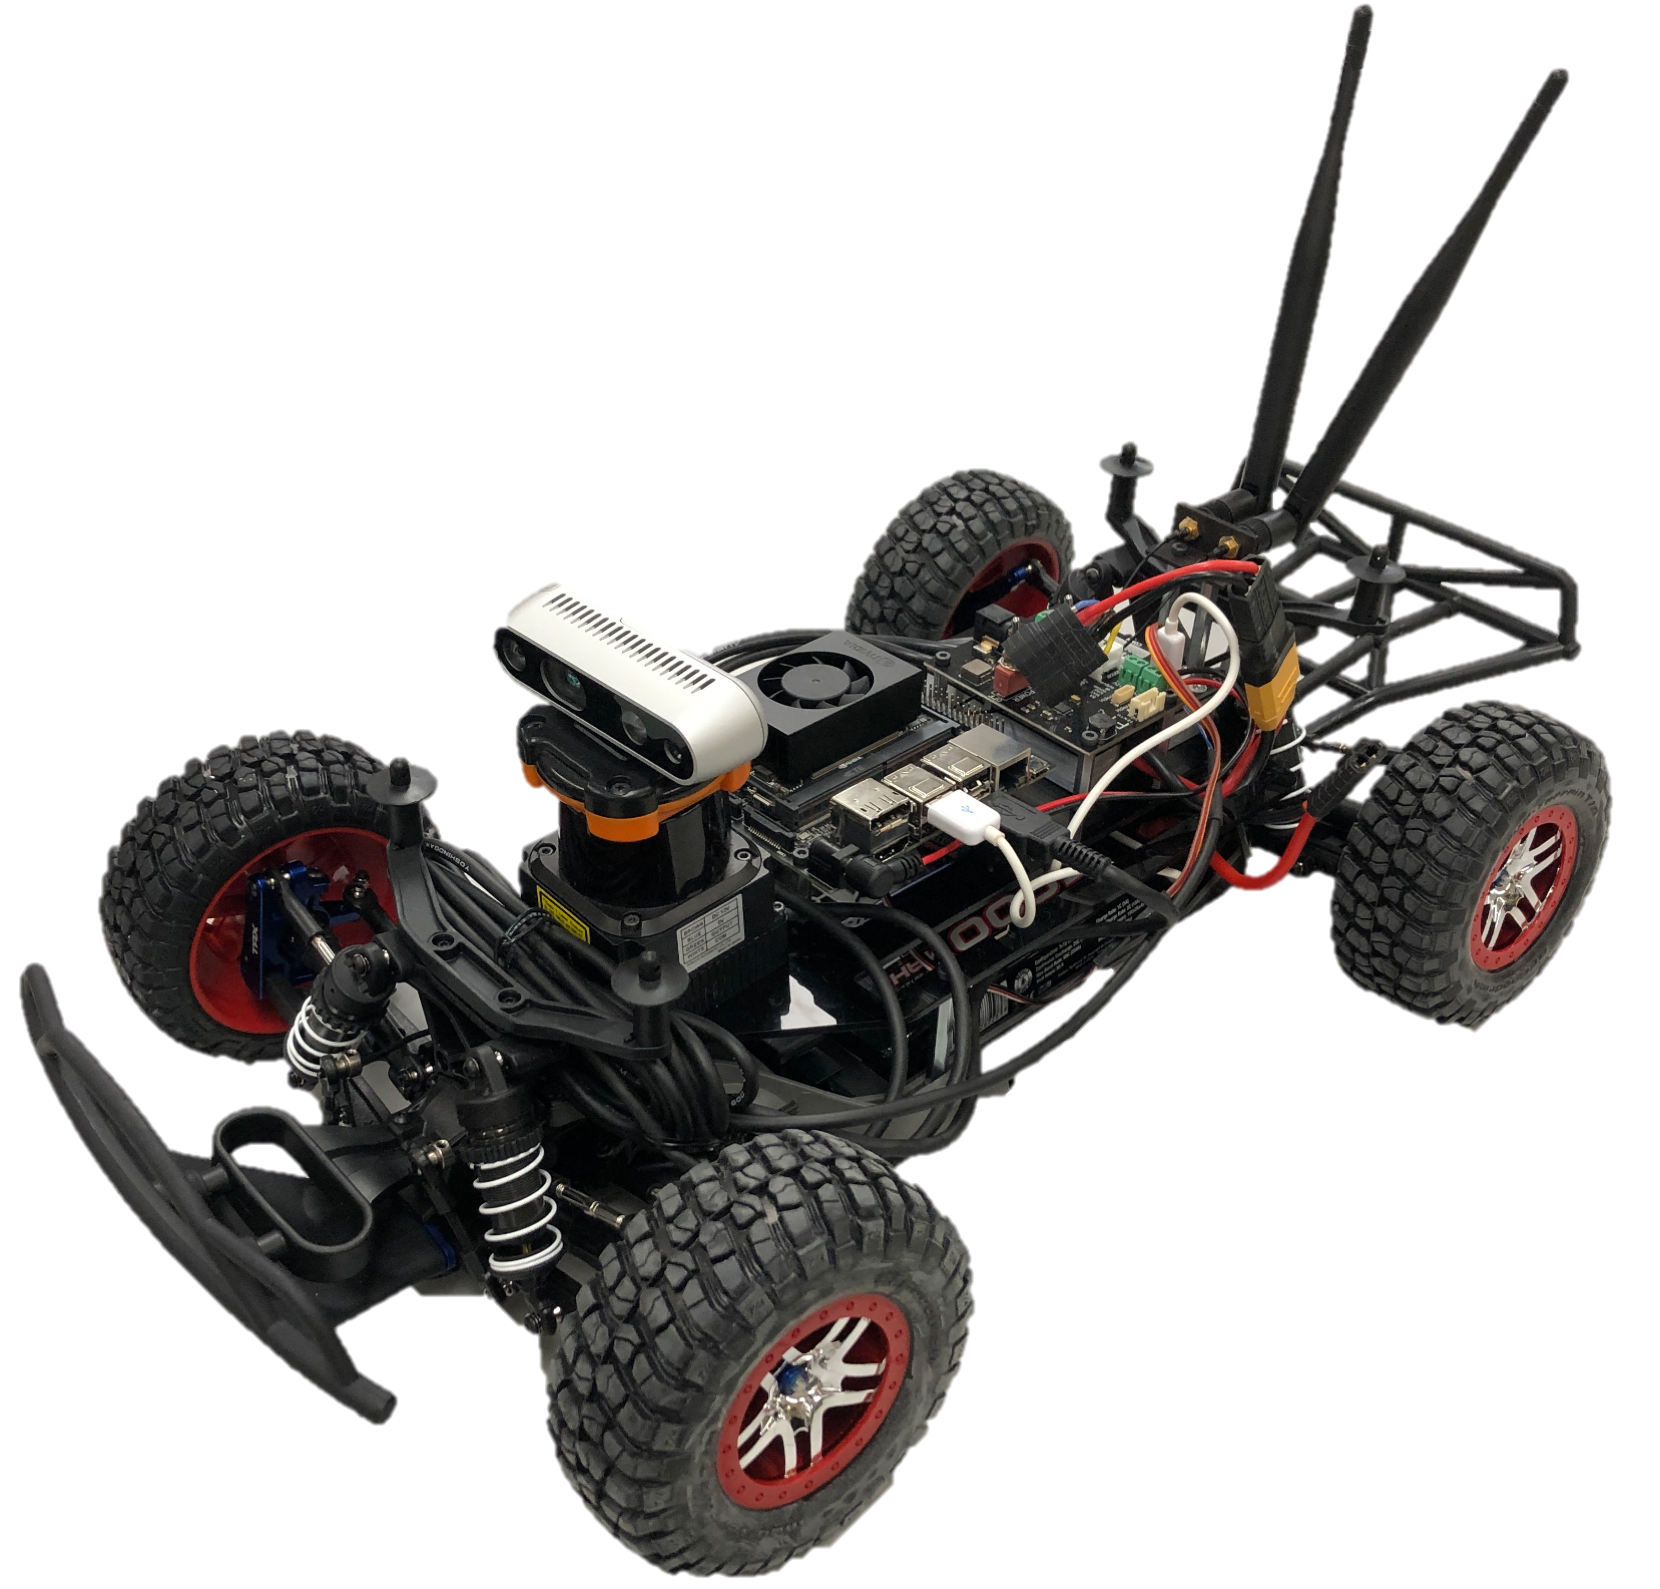
\includegraphics[width=0.2\textwidth]{f1tenth-car.png}
	{\footnotesize \\Robot di F1TENTH \cite{overview}}
\end{wrapfigure}
Oltre a questo, promuove la ricerca nell'ambito della guida autonoma
e altri campi tra cui reinforcement learning, sistemi di comunicazione e robotica;
offre, inoltre, una infrastruttura per costruire l'auto da corsa
e sviluppare il software necessario per farla gareggiare. \cite{f1tenth-web}

La community è stata fondata all'Università della Pennsylvania nel 2016 ma ha iniziato rapidamente
collaborazioni con altre istituzioni e università in tutto il mondo~--~in Italia, alla data di stesura, solo
con l'Università degli Studi di Modena e Reggio Emilia. \cite{f1tenth-about}

\paragraph{Studio preliminare}
Al fine di comprendere al meglio gli argomenti della tesi, è stato effettuato uno studio preliminare su
alcuni macro-argomenti che forniscono le basi fondamentali della guida autonoma e l'utilizzo della
piattaforma di F1TENTH. 
\newpage % da rivedere per non spaccare la lista in più pagine
\noindent Di seguito si elencano le aree tematiche:
\begin{itemize}
	\item Sviluppo con \hyperref[sec:ros]{ROS} e l'ambiente simulatore di
		\hyperref[par:gym]{F1TENTH~gym};
	\item \textbf{Metodi reattivi e dinamiche del veicolo}:\\
		Algoritmo \textit{\hyperref[par:pid]{PID Control}} ed esempio di applicazione in Wall
		following, algoritmo reattivo \textit{Follow the Gap};
	\item \textbf{Mapping \& Localization}:\\
		Localizzazione e mapping simultaneo con \textit{\hyperref[par:slam]{SLAM}} e algoritmo di
		localizzazione \textit{Particle Filter};
	\item \textbf{Planning \& Control}:\\
	      Stack di pianificazione e controllo di un veicolo autonomo, algoritmo di
		  \textit{path tracking} \hyperref[par:pp]{Pure Pursuit}, introduzione ai
	      \textit{local planner} e algoritmi come RRT.
\end{itemize}

\paragraph{F1TENTH gym}
\label{par:gym}
% https://docs.google.com/presentation/d/1zfzzjVTbXNIZ75BFtGEwQBJRHlY95VKkFQjJhYfznpI/edit#slide=id.g1cca33b1c19_0_3213
La community sviluppa e mantiene un simulatore open-source specifico per F1TENTH \cite{f1tenth-gym} in
modo da poter sviluppare e testare comodamente senza l'uso di hardware specifico definito per la
costruzione del robot.\\ Il simulatore permette di definire la dinamica del veicolo in modo tale da avere
una simulazione più reale possibile.

% ================== Autonomous Driving Pipeline =======================
\section{Autonomous Driving Pipeline}
\label{sec:pipeline}
Un progetto ben strutturato è più efficiente da mantenere e ha maggiori probabilità
di funzionare correttamente: ciò si applica anche in questo caso.\\
Un progetto complesso come quello dei veicoli autonomi deve essere suddiviso in sotto-problemi
più specifici e in modo tale che uniti insieme risultino nella soluzione del problema.

\bigskip
\noindent Il \emph{software} per i veicoli autonomi segue un \textit{ciclo} di operazioni
in cui il prodotto di una fase è input della successiva; si identificano in ordine tre fasi:
\begin{enumerate}
\item \textbf{Perception} -- Attraverso sensori ottici e radar si \emph{percepisce} il mondo attorno a sè,
	  ci si localizza nella mappa e si identificano eventuali ostacoli o rivali;
\item \textbf{Planning} -- Stando ai dati generati nella fase precedente,
	  si determinano quali saranno le \emph{mosse future} seguendo delle policy prescritte;
\item \textbf{Control} -- Si generano dei comandi di sterzata e di velocità per attuare le scelte
	  determinate nella fase precedente.
\end{enumerate}

L'input per la prima fase (\textit{Perception}) e l'ouput dell'ultima (\textit{Control})
è direttamente l'hardware: dunque nella prima sono i sensori ottici e radar, come citato precedentemente,
mentre nella seconda sono gli attuatori per i controllo della velocità e angolo delle ruote.

Il risultato che si vuole ottenere, quindi, è quello di una sequenza di comandi di sterzata e
accelerazione in un contesto, quello delle corse, che richiede una certa velocità di esecuzione per poter
essere il più reattivi possibile, per questo motivo è preferibile eseguire il ciclo tra le 20 e 50 volte
al secondo. Una rappresentazione grafica della pipeline intera si trova alla figura~\ref{fig:av-pipeline}.

\begin{figure}[H]
\centering
\caption{Pipeline per i veicolo autonomi \cite{overview}}
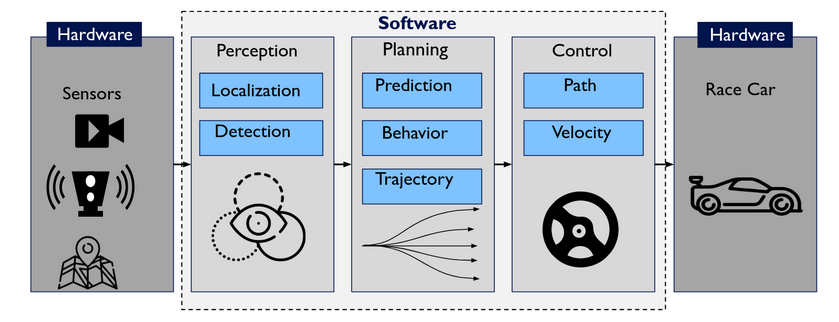
\includegraphics[width=\textwidth]{AV-pipeline.png}
\label{fig:av-pipeline}
\end{figure}

Di seguito si analizzano più nel dettaglio le fasi sopra citate.
\subsection{Perception} 
La prima fase ha il compito di \textit{analizzare} i dati prodotti da diversi tipi di sensori come quelli
ottici, laser e IMU (Inertial Measurment Unit) e ha come obiettivi quelli di: \cite{betz2022autonomous}
\begin{itemize}
	\item determinare l'ambiente statico, chiamato anche \textit{mappa}, che in questo contesto
	      rappresenta i confini del tracciato in cui il robot gareggia;
	\item eventuali ostacoli o altri robot rivali, che quindi compongono la
	      parte dinamica; 
	\item \textit{localizzarsi} all'interno della mappa, ovvero
	      determinare posizione e orientamento del robot rispetto alla mappa.
\end{itemize}
In questa fase, quindi, si ritrovano algoritmi di object detection -- di cui però non è stato argomento
di studio per questa tesi -- algoritmi di mapping e localization, come Particle Filter e SLAM
(\textit{S}imultaneous \textit{L}ocalization \textit{A}nd \textit{M}apping).

\paragraph{Localization}
% https://docs.google.com/presentation/d/1EAzm9A7FbAZFmA8l3ZNb2qjY_GqrLP0r-0uYwL0lLfs/edit#slide=id.g11505ea6fbe_0_901
Sebbene possano essere sfruttate tecnologie come il GPS, la ricerca nelle corse autonome si concentra
maggiormente su una soluzione che richieda solo l'uso di sensori ottici, laser e odometria.
\cite{betz2022autonomous} Per effettuare la localizzazione del robot è necessario avere un modello della
mappa.

Una prima soluzione potrebbe essere quella di partire da una posizione nota e di calcolare la posizione
successiva integrando le misurazioni dei vari sensori e l'odometria delle ruote: questa tecnica viene
chiamata \textit{Dead Reckoning} e, sebbene possa funzionare correttamente in un simulatore, nella realtà
le misurazioni dei sensori contengono del rumore e l'odometria delle ruote generalmente non ha la
precisione richiesta per via di un possibile slittamento delle ruote stesse: tutto ciò, quindi, introduce
nei calcoli degli \textit{errori} che si accumulano col tempo, portando a risultati errati.

La soluzione è quella di rendere più robusti i calcoli tenendo conto del rumore dell'odometria e dei
sensori e compensare alla mancanza di informazioni riguardo la posizione iniziale. Gli algoritmi
modellano questo aspetto usando il \textit{calcolo delle probabilità}. I principali sono: il già citato
Particle Filter, noto anche come AMCL (Adaptive Monte Carlo Localization) e principale algoritmo di
localization usato nello studio di questa tesi e nei laboratori, filtro di Bayes e derivati come Kalman
filter.

\paragraph{SLAM}
\label{par:slam}
SLAM è una tecnica che consente ai robot di eseguire simultaneamente la localizzazione e il mapping
di un ambiente sconosciuto. Siccome i problemi di mapping e localization necessitano l'uno dell'altro
per per poter essere risolti, è necessario risolverli contemporaneamente se non si hanno dati
nè sull'ambiente nè sulla posizione del robot.\\
Ad alto livello, l'algoritmo segue questi passaggi:
\begin{enumerate}
	\item \textit{prima scansione}: si usa la prima scansione come mappa iniziale;
	\item \textit{cambio della posizione}: il robot si muove di una certa quantità in un piccolo
	      lasso di tempo, si registra quindi una nuova scansione della mappa;
	\item \textit{stima della posizione}: la nuova scansione viene correlata con la mappa per
	      stimare il cambiamento di posizione;
	\item \textit{aggiornamento della mappa}: si integra la nuova scansione nella costruzione della mappa
	      sovrapponendo le misurazioni.
\end{enumerate}

\subsection{Planning}
La fase di Planning è stata argomento di studio approfondito di questa tesi, perciò verrà descritta
completamente nel Capitolo~\ref{chap:plan} a pag.~\pageref{chap:plan}.

\subsection{Control}
La terza fase prevede di attuare le decisioni calcolate nella fase di planning: deve quindi generare, in
questo contesto, dei controlli di accelerazione e angolazione delle ruote. In realtà questa fase rientra
in un più vasto e più generale campo di studi: l'\textit{ingegneria del controllo} (o dell'automazione).\\
I principali problemi che bisogna affrontare in questa fase sono:
\begin{itemize}
	\setlength\itemsep{0em}
	\item[$-$] come seguire una traiettoria data?
	\item[$-$] come compensare gli errori degli attuatori?
	\item[$-$] come guidare il più velocemente possibile?
\end{itemize}
Si fanno distinzione di due tipologie di algoritmi di controllo: gli \textit{open-loop} e
\textit{closed-loop}, chiamati anche feedback. In questo contesto, la differenza tra i due è che la
seconda tipologia di algoritmi riceve in input, appunto in \textit{feedback}, anche lo stato corrente del
veicolo rispetto agli output di controllo generati precedentemente; in questo modo è possibile calcolare
l'errore tra il comando calcolato e l'effettivo risultato dell'applicazione di quel comando dagli
attuatori, così da poterlo compensare al prossimo comando inviato.

\paragraph{PID Controller} \cite{lection04, pid-wiki}
\label{par:pid}
L'algoritmo più conosciuto, specialmente per la sua semplicità, è il \textit{PID Controller} che viene
usato ampiamente in tutta l'industria dell'ingegneria del controllo, non solo in questo contesto.\\
PID è un acronimo che sta per \textbf{P}roportional-\textbf{I}ntegral-\textbf{D}erivative e questo
suggerisce che l'ouput è calcolato secondo tre parametri. Si tratta di un algoritmo closed-loop.

Con \textbf{proporzionale} si intende che il comando generato deve essere proporzionale all'errore tra lo
stato corrente del robot e lo stato desiderato.
Siccome ci si vuole che l'errore diminuisca col tempo, con \textbf{derivativo} si intende che si applica
una correzione all'ouput che è proporzionale alla velocità con cui l’errore si riduce.
Infine, con \textbf{integrale} si applica un'ulteriore correzione calcolata sia dalla magnitudine
dell'errore sia dalla sua durata nel tempo, ovvero si correggono gli errori accumulati nel tempo che
avrebbero dovuto essere corretti prima.

\paragraph{Pure Pursuit} \cite{lection10}
\label{par:pp}
Un'altro algoritmo closed-loop più specifico per le corse di robot è Pure Pursuit. In questo caso, il
problema richiedere una sequenza di waypoint, ovvero punti nella mappa che formano un \textit{tracciato},
che il robot deve seguire. L'algoritmo tiene conto della dinamica del veicolo, che in questo caso è
\textit{non-holonomic}, quindi calcola l'arco che congiunge il robot e il primo waypoint che si trova ad
una distanza prefissata, il lookahead, dalla macchina.\\
Questo è stato il principale algoritmo usato nei laboratori e nello studio della tesi, seppur con qualche
modifica migliorativa.


% ================== ROS 2 ================================
\section{ROS2}
\label{sec:ros}
% cit: https://docs.ros.org/en/humble/Citations.html
% https://www.ros.org/blog/ecosystem/
% https://www.ros.org/blog/why-ros/
% https://www.ros.org/blog/getting-started/#
% https://index.ros.org/packages/
% http://design.ros2.org/articles/changes.html ros1 vs ros2
ROS è un acronimo che sta per \textbf{R}obot \textbf{O}perating \textbf{S}ystem e,
sebbene il nome possa trarre in inganno, non è un sistema operativo nel senso tradizionale,
bensì si presenta come un mediatore -- un \textbf{middleware} -- tra l'applicazione robot
e l'hardware del robot, ma non sostituisce il sistema operativo sottostante. \cite{ros-ecosystem}\cite{scirobotics}

Viene usato da tutta l'industria della robotica per via della sua alta modularità:
dalla ricerca all'insegnamento, da progetti di un gruppo di persone a progetti più importanti
di grosse aziende. ROS fornisce i \textit{building blocks} da usare così da facilitare e velocizzare
la realizzazione dell'applicativo e fornisce un metodo di comunicazione efficiente tra le varie componenti.

Il progetto è \href{https://github.com/ros}{\textit{open-source}} ed ha una grossa community di
sviluppatori e ricercatori internazionale che lo mantiene e distribuisce pacchetti integrativi per
diverse funzionalità come driver per i sensori e attuatori, algoritmi noti, compatibilità con altri
programmi, visualizzazioni in tempo reale e tante altre funzioni di utilità. In questo senso, ROS si
presenta più simile a un \textit{SDK} (Software Development Kit) accompagnato da una serie di tools,
principalmente a linea di comando.

ROS viene rilasciato con la stessa filosofia delle \textit{distro linux}, con più distribuzioni mantenute
nello stesso tempo. Va notato che le differenze tra ROS e ROS2 sono profonde differenze
di design e aggiornamento delle tecnologie come, per esempio, l'aggiornamento dei linguaggi supportati,
il sistema di build e importanti modifiche alla gestione dei \hyperref[ros:msgs]{messaggi} e servizi. \cite{ros-diff}
Attualmente, ROS e ROS2 supportano due linguaggi: C++ e Python. In questa tesi è stato usato Python.
Durante lo studio di questa tesi è stato usato ROS2, distribuzione
\href{https://docs.ros.org/en/humble/}{\textit{"Humble"}}, per necessità di compatibilità con alcuni
pacchetti.

\bigskip
\noindent ROS, fondamentalmente, fornisce un metodo di comunicazione tra le componenti dell'applicativo,
che vengono chiamati \hyperref[ros:nodes]{\textbf{\textit{Nodi}}}, attraverso diversi sistemi tra cui i
\hyperref[ros:topics]{\textbf{\textit{Topic}}}, i \hyperref[ros:srv-act]{\textit{Servizi} e le
\textit{Azioni}}. L'insieme dei nodi e dei loro collegamenti formano il \textit{ROS~Graph}, il grafo dei
nodi.

\medskip
\begin{figure}[h]
	\centering
	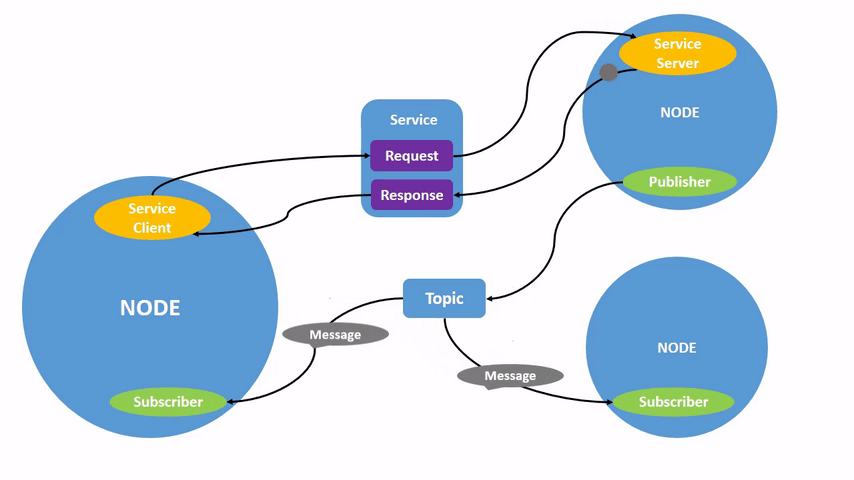
\includegraphics[width=1\textwidth]{ros-topic-srv.png}
	\caption{Esempio di ROS Graph \cite{lection01}}
	\label{fig:ros-topic-srv}
\end{figure}
\noindent Di seguito si analizzano le componenti principali di cui ROS è composto.
% https://docs.ros.org/en/iron/Concepts/Basic.html
\paragraph{Nodi \cite{undr-nodes, ros-nodes}} 
\label{ros:nodes}
% https://docs.ros.org/en/iron/Tutorials/Beginner-CLI-Tools/Understanding-ROS2-Nodes/Understanding-ROS2-Nodes.html
% https://docs.ros.org/en/iron/Concepts/Basic/About-Nodes.html
I nodi, \textit{Nodes} in inglese, sono l'unità computazionale che partecipa al ROS Graph;
idealmente, un nodo dovrebbe essere responsabile di un solo compito, logicamente separato
da altri altri, per esempio controllare le ruote, processare i dati grezzi derivati dalle misurazioni
dei laser o implementare un algoritmo come Pure Pursuit.
Un completo sistema robotico comprende, quindi, un insieme di nodi che lavorano congiuntamente, spesso
contenuti nello stesso eseguibile.\\

\paragraph{Topic \cite{undr-topics, ros-topics}}
\label{ros:topics}
% https://docs.ros.org/en/iron/Concepts/Basic/About-Topics.html
% https://docs.ros.org/en/iron/Tutorials/Beginner-CLI-Tools/Understanding-ROS2-Topics/Understanding-ROS2-Topics.html
I topic sono il principale strumento con cui i nodi di un ROS Graph si \textit{scambiano dati}.
I topic sono entità \textbf{\textit{fortemente tipizzate}} che implementano
un pattern \textbf{\textit{publisher/subscriber}} di tipo \textit{anonimo}, ciò significa
che i nodi conoscono una interfaccia comune con cui scambiarsi messaggi ben definiti.\\
\textit{Anonimo} significa che chi invia o riceve dei messaggi da o verso un topic
non ha modo di identificare mittente o destinatario perché, in questo contesto, non ha una grossa rilevanza,
sebbene esistano comunque dei modi per scoprirlo; inoltre, ogni messaggio generato da un publisher
viene ricevuto da ogni subscriber, nell'idea che un nodo si sottoscriva a un topic solo se ne è
interessato; questo ha il vantaggio di una grossa flessibilità in termini di manuntenibilità.\\
I nodi possono \textit{pubblicare} e \textit{sottoscriversi} ad un numero arbitrario di topic
per inviare e ricevere dati da altri componenti del grafo: si può avere quindi una relazione uno a
uno, uno a molti, molti a uno e molti a molti.\\
I topic vengono identificati da una stringa univoca che ne rappresenta il nome.

\paragraph{Messaggi \cite{ros-message}}
\label{ros:msgs}
% https://docs.ros.org/en/iron/Concepts/Basic/About-Interfaces.html#messages
I messaggi sono l'\textit{interfaccia}, agnostica al linguaggio, con la quale i \hyperref[ros:nodes]{nodi}
comunicano tra di loro. Descrivono un tipo di dato strutturato \textbf{fortemente tipizzato} in un
file con estensione \verb|.msg|. Questo tipo di file contiene una lista di attributi definiti da
tipo dell'attributo, nome ed eventuale valore di default. Il tipo può essere un tipo base
(\verb|short|, \verb|double|, \verb|string|) o un tipo composto, ovvero un'altro tipo messaggio.

\paragraph{Parametri e Launch files \cite{ros-params, ros-launch}}
% https://docs.ros.org/en/humble/Concepts/Basic/About-Launch.html
% https://docs.ros.org/en/humble/Concepts/Basic/About-Parameters.html
É possibile parametrizzare i nodi in modo da configurarli sia all'avvio sia durante l'esecuzione
senza cambiare codice e ricompilarlo. I parametri consistono in una coppia chiave-valore ed una
opzionale descrizione, che può indicare eventuali vincoli di tipo e range di valori.\\
Spesso i parametri vengono inizializzati all'avvio del nodo attraverso quelli che vengono chiamati
\textit{launch file} usati col comando \verb|ros2 launch| e che quindi permettono di avere \textit{diverse
configurazioni dello stesso nodo} senza doverlo ricompilare. Un'altro caso d'uso è durante la fase di
tuning per alcuni algoritmi: se il contesto lo permette è possibile modificare online i valori dei
parametri (per esempio da CLI), a patto che venga gestito nel codice del nodo.
I launch file possono essere usati anche per avviare più nodi contemporaneamente, in modo da
automatizzare l'intero applicativo.

\paragraph{Services e Actions \cite{ros-services, ros-actions}}
\label{ros:srv-act}
% https://docs.ros.org/en/humble/Concepts/Basic/About-Actions.html
% https://docs.ros.org/en/humble/Concepts/Basic/About-Services.html
Altri due sistemi di comunicazioni fra \hyperref[ros:nodes]{nodi} sono i Servizi e le Azioni.
Questi sono sostanzialmente chiamate remote -- ovvero ad altri nodi -- a procedure seguendo il paradigma
client/server. La loro principale differenza è concettuale e si discrimina dalla velocità di esecuzione:
nei servizi, infatti, la risposta deve essere rapida, mentre nelle azioni ci si aspetta una esecuzione
più lunga, anche di minuti, e si ha la possibilità di cancellarla prima del suo termine.
Entrambi vengono definiti con strutture simili ai messaggi, con file di diversa estensione.

Per citare qualche esempio, nei servizi troviamo operazioni di trasformazioni di coordinate tra frame, mentre
nelle azioni operazioni di più alto livello come \textit{"raggiungi questo waypoint"}.


\bigskip

La figura \ref{fig:ros-topic-srv} rappresenta un ROS Graph comprendente tre nodi, un topic e un servizio;
al topic sono sottoscritti i nodi in basso e ricevono i messaggi prodotti dal nodo in alto a destra che
fa anche da server al servizio da cui riceve richieste dal nodo client.

\section{RViz}
\label{sec:rviz}
RViz (\textbf{R}os \textbf{Vi}suali\textbf{z}er) è il principale strumento di visualizzazione 3D per gli
applicativi ROS. Durante lo studio di questa tesi è stato usato per visualizzare la simulazione di
F1TENTH gym, il modello del robot, la mappa del circuito ed eventuali visualizzazioni dei vari algoritmi
in studio, per esempio i waypoint di goal per Pure Pursuit, l'albero dei punti random generati da RRT e i
waypoint che compongono la raceline ottima.\\
La figura \ref{fig:rviz-example} ne mostra un'esempio.

\begin{figure}[H]
	\centering
	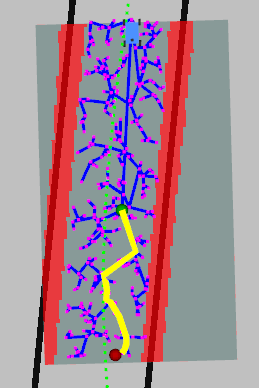
\includegraphics[width=0.4\textwidth, height=0.45\textheight, angle=90]{rrt.png}
	\caption{Esempio di caso d'uso di RViz per visualizzare l'algoritmo RRT}
	\label{fig:rviz-example}
\end{figure}

% Chapter 2

\chapter{Planning}
\label{chap:plan}

In questo capito si andranno ad analizzare i compiti della seconda fase all'interno del ciclo della
\hyperref[sec:pipeline]{pipeline dei veicoli autonomi}, ovvero il planning. In questa fase viene inserito
l'argomento di studio di questa tesi: l'ottimizzazione della traiettoria globale.
Il planning, come suggerisce il nome, ha il compito di pianificare le mosse successive del robot affinché
possa spostarsi in modo ottimale evitando eventuali ostacoli.

\bigskip
\noindent Gli algoritmi si differenziano per tecniche e obiettivi, in particolare si distinguono tre
macro-categorie che rispondono a domande diverse:
\begin{itemize}
	\item Mission/Global Planner: \textit{Qual è l'obiettivo generale del veicolo?} Per esempio trovare
	il percorso più breve, o quello più corto; 
	\item Behavioural Planner: \textit{Come dovrebbe comportarsi il veicolo in diverse situazioni?} Per
	esempio, in una gara con più concorrenti, quando superare un avversario, come e dove;
	\item Local Planner: \textit{Quali sono le traiettorie possibili dalla posizione attuale al goal?}
	Per esempio trovare la miglior traiettoria tale che rientri nella possibilità fisica del veicolo.
\end{itemize}
L'oggetto di questa tesi, l'ottimizzazione della traiettoria di corsa, rientra nella prima categoria.

% Tra i diversi algoritmi presenti in questo ambito si presenta una distinzione tra diverse
% caratteristiche.

\paragraph{\textit{Workspace} vs \textit{Configuration Space}} \ \\
Si distinguono due rappresentazioni degli ostacoli e dell'ambiente: il workspace rappresenta tutte le
azioni possibili a un robot, si pensi al volume occupato da tutti i possibili movimenti di un braccio
meccanico, mentre il configuration space, detto anche C-space, rappresenta tutte le possibili
configurazioni di una data definizione di stato. In questo contesto, all'atto pratico, ciò si traduce che
nel secondo la rappresentazione dell'ambiente e degli ostacoli tiene già conto della dimensione del
robot e quindi quest'ultimo può essere considerato come un singolo punto, mentre ciò non accade nel
primo. La figura \ref{fig:work-vs-conf-space} ne mostra un esempio.

\begin{figure}[H]
	\begin{center}
		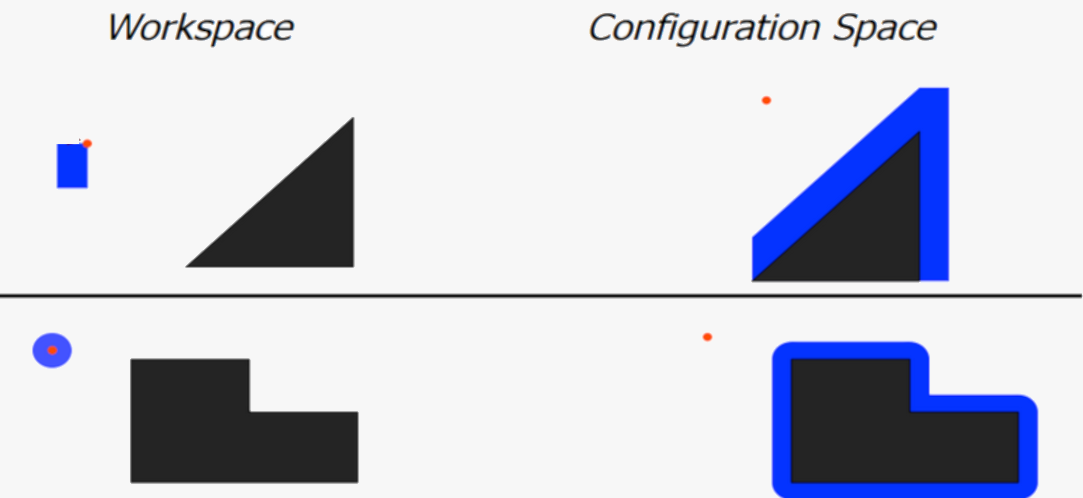
\includegraphics[width=0.95\textwidth]{work-vs-conf-space.png}
	\end{center}
	\caption{Differenze tra Workspace e C-Space \cite{lection11}}
	\label{fig:work-vs-conf-space}
\end{figure}

Nel contesto delle corse si preferisce l'uso del C-space per via della usa espressività nella descrizione
dello stato, che può non solo descrivere un piano o uno spazio tridimensionale, ma è possibile esprimere
ulteriori variabili come la velocità e l'orientamento: è così possibile esprimere ulteriori vincoli.

\bigskip
\noindent Di seguito si analizzano le tre macro-categorie sopra citate.

\section{Local Planner}
L'obiettivo principale del local planner è quello pianificare i movimenti del robot fino ad un dato
orizzonte finito evitando collisioni con l'ambiente ed eventuali avversari. Gli algoritmi si
differenziano per tre categorie principali di risoluzione:
\begin{enumerate}
	\item Applicando modifiche la raceline globale; 
	\item Generando diverse traiettorie vincolate alla dinamica del robot e scegliendo quella migliore;
	\item Campionando lo spazio libero e trovando un percorso attorno agli ostacoli.
\end{enumerate}
Nella prima categoria rientrano, generalmente, algoritmi che si basano su MPC che, sebbene sia un
algoritmo di controllo ottimale, può essere adattato e utilizzato per ricercare il percorso ottimo per
evitare un ostacolo o per migliorare la traiettoria della raceline globale di riferimento in base alla
posizione attuale del veicolo.

Nella seconda categoria ricadono algoritmi che calcolano, fino a un dato orizzonte temporale, lo stato
successivo del veicolo per diversi input di accelerazione e angolo delle ruote; questo operazione produce
diverse traiettorie, dinamicamente corrette per il robot, da cui si sceglie la migliore secondo una
funzione di costo. Altri algoritmi, come State Lattice, generano punti equidistanti nell'ambiente tra di
loro connessi da delle \hyperref[par:spline-def]{spline} che seguono la dinamica del veicolo, poi viene
ricercato il percorso migliore. Un esempio grafico è mostrato in figura \ref{fig:state-lattice}.

La terza categoria, data una occupancy grid e un punto di goal, algoritmi come PRM (Probabilistic Road
Map) e derivati come RRT (Rapidly-Exploring Random Tree) campionano lo spazio libero e generano un grafo
che connette i punti campionati per poi cercare il percorso che avvicina il robot al goal. RRT è stato un
caso di studio durante questa tesi durante un laboratorio del Modulo D. Un esempio di RRT si può trovare
alla figura \ref{fig:rviz-example}. Altre soluzioni usano i classici algoritmi di ricerca su grafo, come
A* e Dijkstra, sulla stessa occupancy grid; il grafo costruito a partire da essa esprime sui nodi le posizioni
nell'ambiente e gli archi i possibili input da quelle posizioni. Queste ultime sono soluzioni discrete,
molto semplici da implementare ma che non hanno la stessa espressività dei metodi continui e che non
hanno la possibilità di descrivere la dinamica del robot.

\begin{figure}[h]
	\begin{center}
		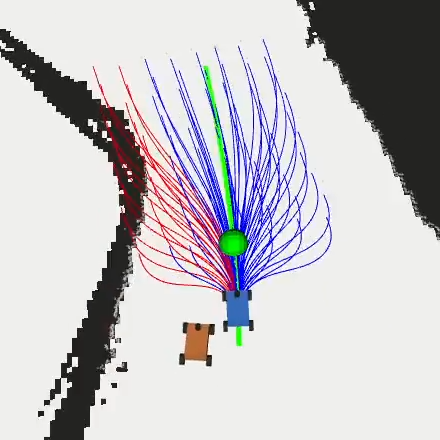
\includegraphics[width=0.5\textwidth]{state-lattice.png}
	\end{center}
	\caption{Esempio grafico dell'algoritmo State Lattice \cite{state-lattice}}
	\label{fig:state-lattice}
\end{figure}

\section{Behavioural Planner}
Il focus di questo planner è generalmente selezionare un peso appropriato a diversi obiettivi o combinare
il risultato del local planner con metodi della teoria del gioco così da pianificare delle mosse atte a
impedire il progresso degli avversari.

Nel primo caso, gli obiettivi rappresentano valori come il progresso sul circuito, la vicinanza con gli
ostacoli e contendenti, la deviazione dal percorso ottimale, la velocità massima; il costo totale di una
traiettoria viene quindi calcolato combinando secondo vari pesi gli obiettivi presi in considerazione,
viene quindi scelto la traiettoria col costo minore.

Nel secondo caso vengono sfruttate metodologie della teoria dei giochi per trovare l'azione migliore in
un ambiente con due o più giocatori. Il problema viene trasformato in gioco competitivo asincrono dove un
singolo giocatore può "muoversi" per volta. Questi approcci spesso includono nel calcolo della soluzione il
concetto di \textit{regret} per trovare la migliore risposta per vincere la gara.

\section{Global Planner}
Come citato più volte precedentemente, questa tipologia di planner è stato oggetto di studio di questa
tesi e quindi ha dedicato un capitolo, il numero \ref{chap:opt} (pag. \pageref{chap:opt}).

Il global planner ha una visione d'insieme del circuito ed è agnostico alla singola gara, perciò i suoi
obiettivi sono legati a proprietà della traiettoria (globale) da seguire; generalmente l'obiettivo
principale è eseguire il tracciato in meno tempo possibile, ma esistono altre possibilità come il minor
consumo d'energia e traiettorie con particolari proprietà geometriche, come la minor curvatura.


% Chapter 3
% ======================================================================

\chapter{Raceline Optimization}
\label{chap:opt}

Lo studio di questa tesi si è concentrato a trovare una soluzione al seguente problema: \textit{data una
mappa, trovare la sua raceline globale ottima, secondo un criterio scelto}. Il
criterio di ottimizzazione principale, in questi casi, è il tempo di percorrenza del tracciato, ovvero il
\textit{lap time}.

Le porzioni interessanti di un circuito da gara sono le \textit{curve}: ne esistono di diversi tipi e
altrettanti modi per affrontarle in base al tipo; trovare una percorso ottimo, in questo senso, è un
compito complesso e il percorso più breve non coincide necessariamente con quello che richiede meno
tempo, a causa delle curve che riducono la velocità media. Una possibile strategia per mantenere alta la
velocità in curva è quella di percorrere la traiettoria con la curvatura minore. Questo approccio,
tuttavia, non prende in considerazione una sequenza di curve e la velocità di uscita da una curva. Il
percorso ottimo in termini di tempo, quindi, è un compromesso tra queste due strategie, ovvero quella che
minimizza la distanza percorsa mantenendo alta la velocità nelle curve ed eventualmente anche in uscita
da esse.

Trovare la raceline ottima è generalmente un'operazione preliminare alla gara, dunque \textit{non può
considerare} eventuali avversari o ostacoli dinamici; per questo motivo viene calcolata nell'assunzione
di un \textit{singolo robot} sul tracciato.
Tuttavia non è utile solo nel contesto considerato: la raceline globale, avendo una visione intera sulla
mappa, può essere sfruttata da un local o behavioural planner come linea guida.

% ================== Le Curve ==========================================
\section{Le curve}
Le principali complessità di un circuito di cui l'ottimizzazione si occupa è come affrontare le curve.\\
Caratteristica principale di una curva è il suo \textit{raggio}: un raggio maggiore corrisponde a
velocità più alte e viceversa; inoltre, si distinguono il raggio esterno e quello interno e la loro
differenza risulta nell'ampiezza del circuito in quel punto.
Esistono anche caratteristiche di natura tridimensionale, come la variazione dell'altezza e
l'inclinazione, tuttavia non sono state oggetto di studio in questa tesi dal fatto che il contesto di
F1TENTH non include questa variabilità, come invece accade nelle gare di F1.

In linea generale, una curva può essere suddivisa in \textit{quattro sequenze} principali, come mostrato
in figura \ref{fig:geom-raceline}:
\begin{enumerate}
	\item approccio e decelerazione;
	\item inizio della curva;
	\item raggiunta dell'apice;
	\item uscita della curva e accelerazione.
\end{enumerate}
Anche la traiettoria, dato che segue una curva, può essere definita con un raggio che può essere
\textit{costante} o \textit{variabile} dall'inizio della curva fino alla fine.

\begin{figure}[H]
	\begin{center}
		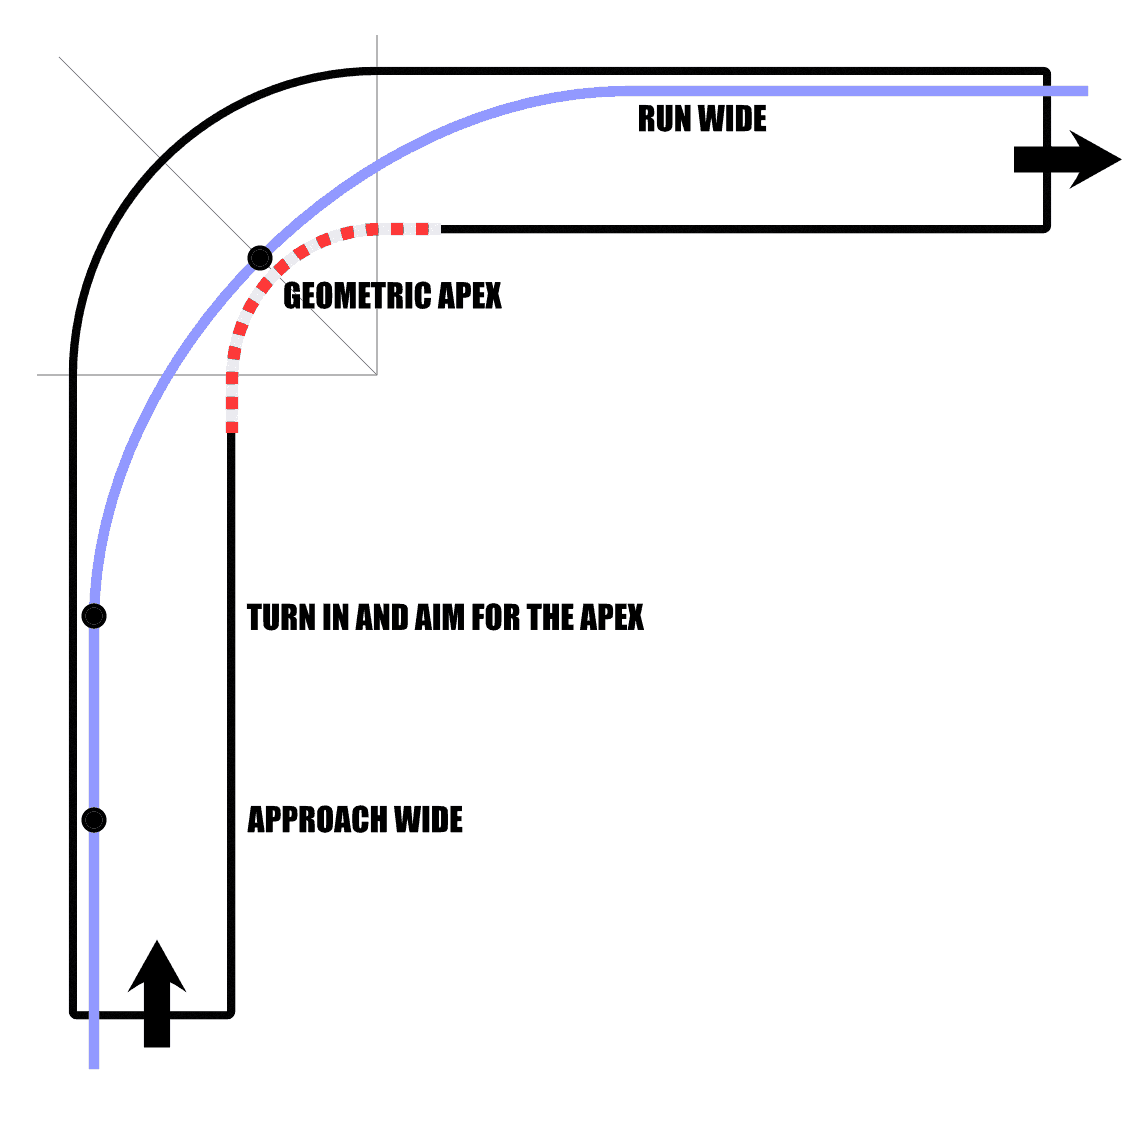
\includegraphics[width=0.65\textwidth]{geometric-apex.png}
	\end{center}
	\caption{Rappresentazione delle fase di una raceline geometrica per una curva a destra \cite{drivingfast}}
	\label{fig:geom-raceline}
\end{figure}

\paragraph{Raceline geometrica}
L'approccio più semplice e immediato per affrontare una curva genera una raceline che prende il
nome di \textit{raceline geometrica}. La strategia prevede queste sequenze, rappresentate in figura
\ref{fig:geom-raceline}:
\begin{enumerate}
	\item approccio largo e verso l'esterno del circuito;
	\item sterzata verso il centro del raggio interno della curva;
	\item uscita larga e verso l'esterno del circuito.
\end{enumerate}
Si tratta, quindi, di una raceline a raggio \textit{costante}.\\
I principali vantaggi di questo approccio rispetto alla raceline ottima sono la sua semplicità, sia in
termini di modellazione sia in termini di computazione, e la possibilità di mantenere un'alta velocità
durante la curva. Tuttavia, la raceline geometrica ha importanti svantaggi quali una decelerazione
prematura all'entrata della curva, una accelerazione ritardata all'uscita e la possibilità di ritrovarsi
in uno stato svantaggiato per affrontare la prossima curva, nel caso di curve in sequenza.

Dunque, la raceline ottimale non dovrebbe tener conto solamente della singola curva ma eventualmente
anche di quelle successive: per estensione, quindi, deve essere considerato tutto il circuito.

\paragraph{Raceline ottimale}
Al contrario della raceline geometrica, non è possibile definire a priori le sequenze da seguire come
fatto in precedenza, proprio perché dipende dalle caratteristiche della curva.
Riprendendo come esempio la curva in figura \ref{fig:geom-raceline}, la raceline ottimale -- ovvero quella
che riesce ad eseguire la curva nel minor tempo possibile -- tarda il più possibile l'inizio della curva
per mantenere più velocità all'entrata, decelera più velocemente e ha una virata più stretta e con un
apice più distante da quello geometrico, così facendo si ha la possibilità di aver più tempo per
accelerare di nuovo all'uscita della curva con la possibilità di mantenere una traiettoria più centrata
rispetto al circuito.

In figura \ref{fig:cmp-lines} vi è una comparazione grafica tra le due raceline.\\
La raceline ottima, inoltre, adegua la traiettoria di uscita in base alla curva successiva, se presente,
in modo tale da affrontarla anch'essa nel modo ottimale. Si nota la distinzione in figura
\ref{fig:cmp-opt-lines}.

\begin{figure}[H]
	\begin{minipage}[c]{0.45\textwidth}
		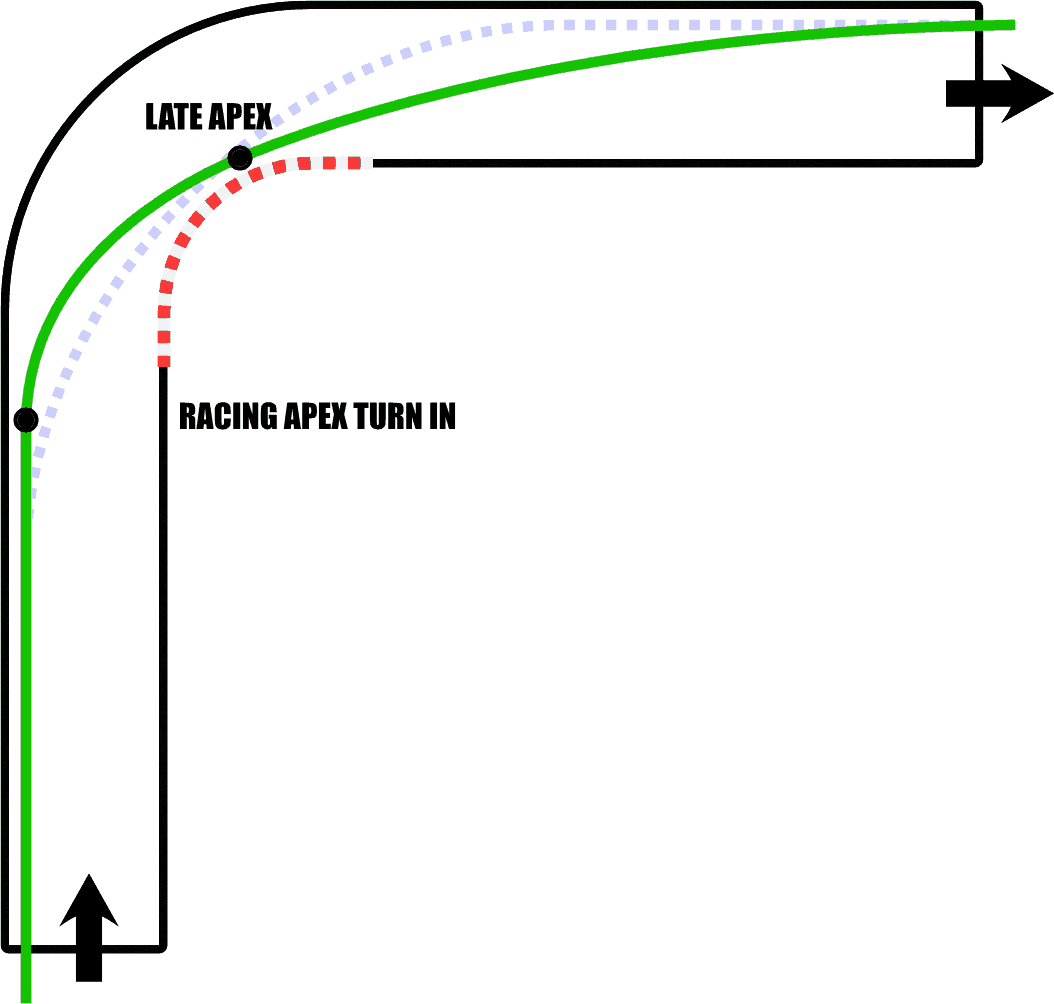
\includegraphics[width=0.80\textwidth]{comparing-lines.png}
		\caption{Comparazione tra raceline ottimale, in verde, e raceline geometrica, in blu
		tratteggiato \cite{drivingfast}}
		\label{fig:cmp-lines}
	\end{minipage}\hfill
	\begin{minipage}[c]{0.45\textwidth}
		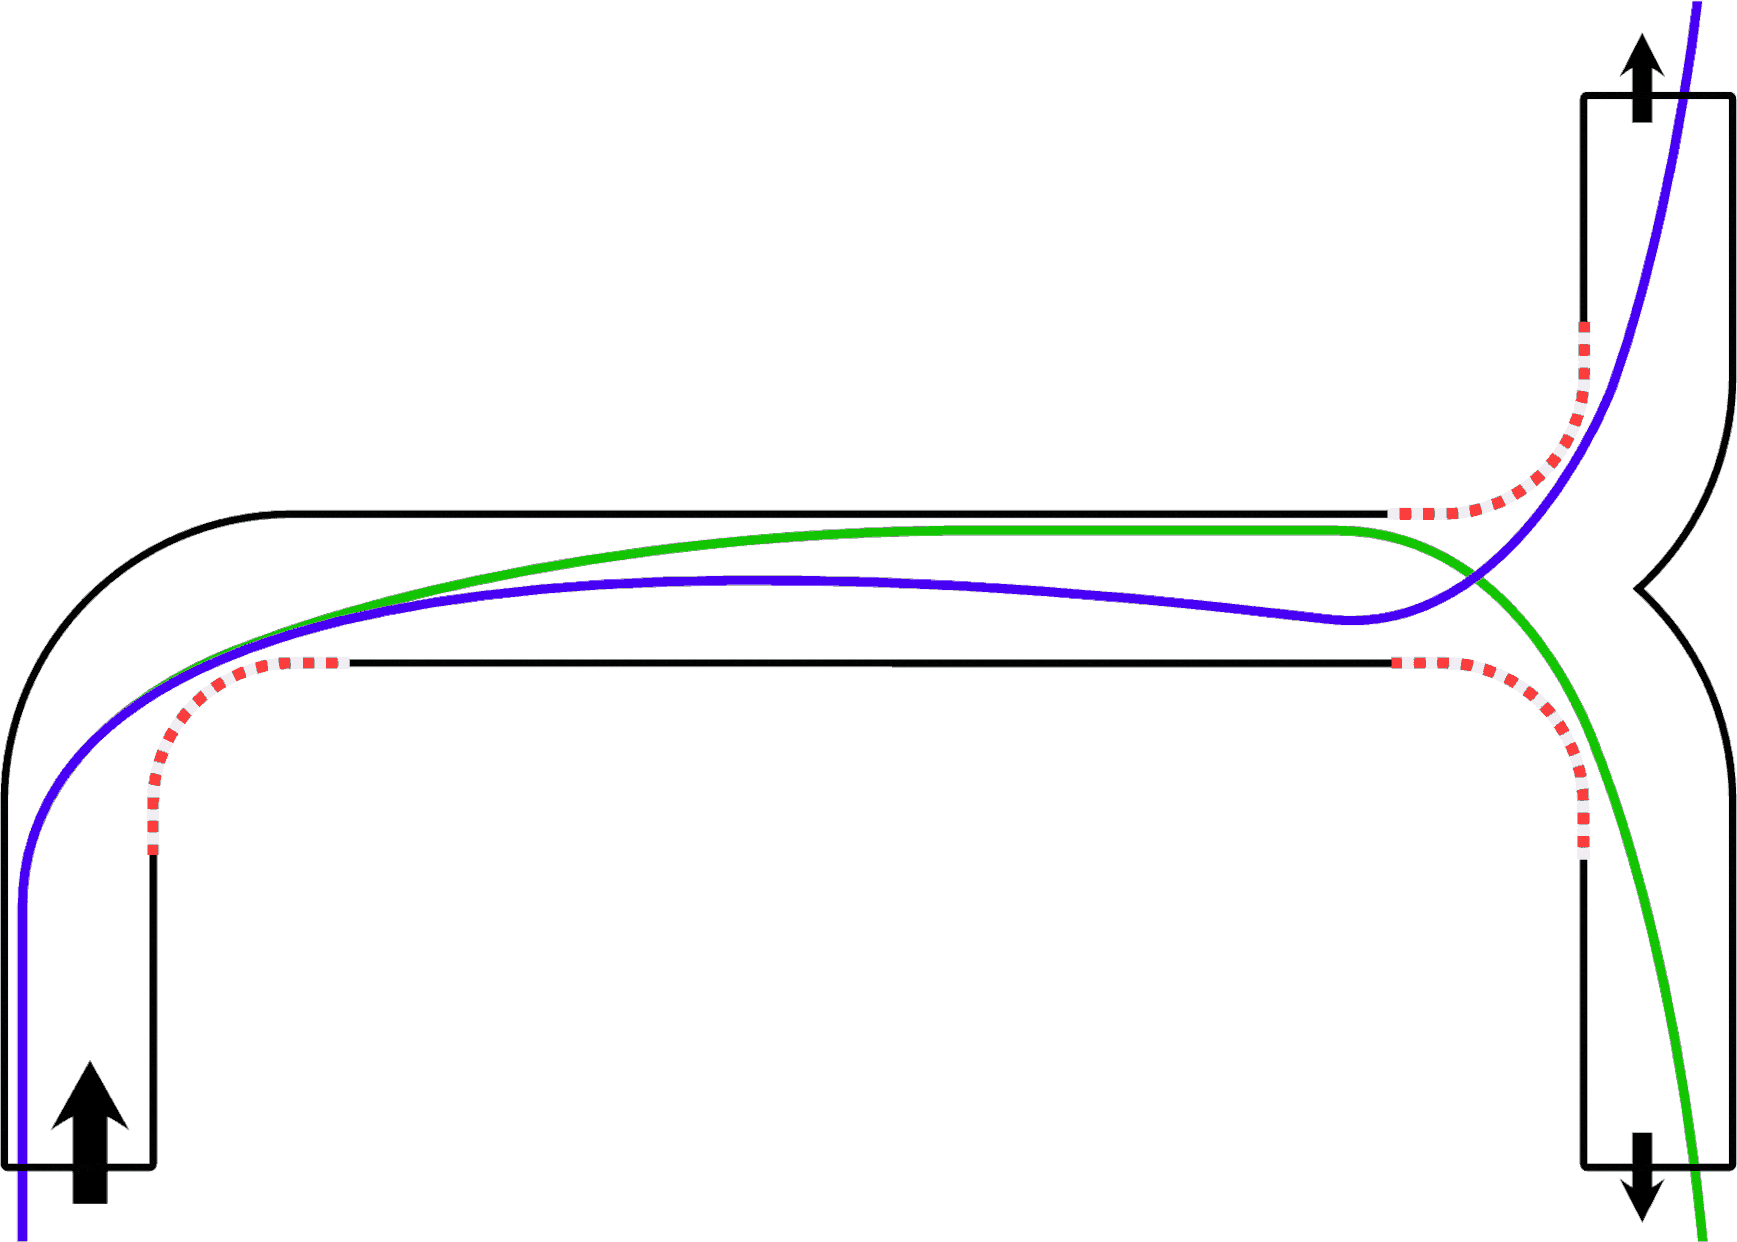
\includegraphics[width=1\textwidth]{multiple-corners.png}
		\caption{\raggedright Confronto tra raceline ottime con due curve distinte in
		sequenza \cite{drivingfast}}
		\label{fig:cmp-opt-lines}
	\end{minipage}
\end{figure}


% ================== Descrizione del problema ==========================
\section{Descrizione del problema}
% Il lavoro è stato basato su questa repo \url{https://github.com/CL2-UWaterloo/Raceline-Optimization}.
% fonti: L22 Raceline-Optimization slide

Di seguito si presentano alcune definizioni più formali dei termini utilizzati precedentemente e il
processo di generazione del percorso ottimo secondo un certo criterio.

\bigskip
\noindent In questa tesi sono state implementate e analizzate tre strategie differenti:
\begin{itemize}
	\setlength\itemsep{0em}
	\item Percorso più breve  -- \textit{shortest path};
	\item Curvatura minima -- \textit{minimum curvature};
	\item Tempo minimo -- \textit{minimum time}.
\end{itemize}

\noindent Il problema in questione è un problema di ricerca su due variabili: il percorso effettivo sulla mappa e
la velocità da mantenere per ogni punto del percorso. Queste due variabili assieme definiscono la
\textit{traiettoria} o \textit{raceline}, in inglese.\\
I vincoli applicati alla ricerca sono due: i limiti dinamici del veicolo, per esempio quanta forza G il
veicolo riesce a sostenere in sterzata, e gli ostacoli statici, rappresentati dai bordi del circuito.

\bigskip
\noindent Il problema viene suddiviso in due sotto-problemi, ovvero risolvere singolarmente la ricerca sulle due
variabili in gioco. Si distinguono quindi, in sequenza:
\begin{enumerate}
	\setlength\itemsep{0em}
	\item Generazione del percorso secondo i vincoli desiderati -- \hyperref[sec:path-models]{\textit{path
		planning}}
	\item Calcolo della velocità sul percorso generato -- \hyperref[sec:velocity-plan]{\textit{velocity
		planning}}
\end{enumerate}
In particolare, il path planning, almeno per quanto riguarda le prime due strategie, viene modellato come
un problema di programmazione quadratica geometrica (Geometric QP), che ha i vantaggi di richiedere pochi
parametri e di essere computazionalmente veloce; esistono anche altri tipi di algoritmi di ottimizzazione
basati su evoluzione, come CMA-ES. Il velocity planning può essere risolto con algoritmi a stato
quasi-stazionario come l'algoritmo forward-backward. Un ulteriore metodo per il velocity planning per il
tempo più breve è descritto in \textit{"Minimum-time speed optimization over a fixed path"}
\cite{lipp2014minimum}.

Per quanto riguarda la terza strategia, i due sotto-problemi devono essere risolti contemporaneamente
usando algoritmi di controllo ottimale, questi hanno la possibilità di includere ulteriori vincoli, come
per esempio limitazioni al consumo di energia o considerare l'attrito delle ruote per diversi terreni e
condizioni meteo.\cite{christ2021time} Sono algoritmi con modelli dinamici dell'auto più completi e
fedeli alla realtà che raccolgono nel problema diverse variabili, per questo sono più complessi e
richiedono più sforzo computazionale, ma hanno il vantaggio di essere più realistici nel risultati
rispetto alle loro controparti modellate in problemi di programmazione quadratica.

\paragraph{Definizione di spline \cite{olausson2021optimal} \cite{globalplanning-lec}}
\label{par:spline-def}
Un percorso, per poter essere computato da una macchina, deve necessariamente essere discretizzato in
punti, detti \textit{samples}.
Tuttavia è necessaria una descrizione matematica del tracciato: questa viene formulata con l'uso delle
\textit{spline}. Una spline è una funzione definita a pezzi da un'insieme di polinomi dello stesso grado
il cui scopo, in questo contesto, è quello di interpolare dei punti, ovvero i samples, in modo tale che
la funzione sia continua fino ad un dato ordine.

Una spline, per poter rappresentare un percorso che deve essere seguito da un'auto, è necessario che
rispetti alcuni vincoli, ovvero:
\begin{enumerate}
	\item L'inizio di un polinomio deve essere un punto di discretizzazione, un sample;
	\item La fine di un polinomio deve essere il sample successivo all'inizio;
	\item L'orientamento alla fine di una funzione deve essere uguale all'orientamento della funzione
	      successiva;
	\item La curvatura alla fine di una funzione deve essere uguale alla curvatura della funzione
	      successiva;
\end{enumerate}
I primi due vincoli sono garantiti dal fatto che la spline interpola i sample, per gli ultime due è
necessario calcolare la derivata prima e seconda del polinomio in quei punti. I polinomi di grado tre
offrono, quindi, una buona rappresentazione del percorso perché garantiscono la calcolabilità delle
derivate prime e seconde per ogni punto del dominio.

Il dominio di ogni polinomio viene normalizzato per la distanza tra il punto di partenza e quello di fine
dal parametro $t$, dove $t = 0$ indica il punto di inizio e $t = 1$ il punto di fine.
Sia $f_i(t) = a_i + b_i t + c_i t^3 + d_i t^3$ il polinomio che ha come inizio il sample all'indice $i$,
l'immagine \ref{fig:spline} mostra graficamente una spline e i vincoli associati.

\begin{figure}
	\begin{center}
		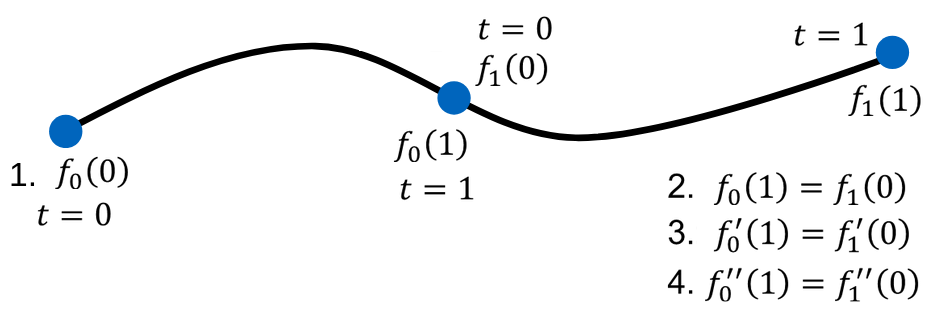
\includegraphics[width=0.95\textwidth]{spline.png}
	\end{center}
	\caption{Esempio di spline formata da due polinomi e vincoli associati \cite{lection22}}
	\label{fig:spline}
\end{figure}
Il calcolo dei valori delle $x$ e delle $y$ avviene separatamente ma usando gli stessi metodi, di
seguito, quindi, verranno descritti solo la formulazione per $x$.
Matematicamente i vincoli sopra descritti vengono formulati come:
\begin{enumerate}
	\item $t = 0 \quad a_i = x_i$
	\item $t = 1 \quad a_i + b_i + c_i + d_i = x_{i+1}$
	\item $t = 1\ \text{e}\ t = 0 \quad b_i + 2 c_i + 3 d_i - b_{i+1} = 0$
	\item $t = 1\ \text{e}\ t = 0 \quad 2 c_i + 6 d_i - 2 c_{i+1} = 0$
\end{enumerate}
dove per il 3. e 4. punto vengono rispettivamente ricavati dalla differenza \\
$f'_i(1) - f'_{i+1}(0)$ e $f''_i(1) - f''_{i+1}(0)$

% Un esempio dell'uso di una spline per interpolare dei punti è mostrato in figura \ref{fig:spline}

\paragraph{Definizione di centerline}
\label{par:centerline}
La centerline, o reference line, è il percorso che è equidistante dai bordi del circuito. Viene
discretizzato in punti di egual distanza tra loro e si registrano le distanze ai bordi destro e sinistro,
così da formare una line immaginaria, ortogonale alla reference line, che unisce i due punti. L'immagine
\ref{fig:centerline-ex} ne mostra un esempio grafico.

La linea centrale di riferimento è necessaria agli algoritmi di ottimizzazione come punto di partenza per
trovare la soluzione ottima.
La distanza dei samples è un parametro dell'algoritmo e deve essere decisa in base al caso d'uso, come
approfondito al paragrafo \ref{par:tuning}.

\begin{figure}[h]
	\begin{center}
		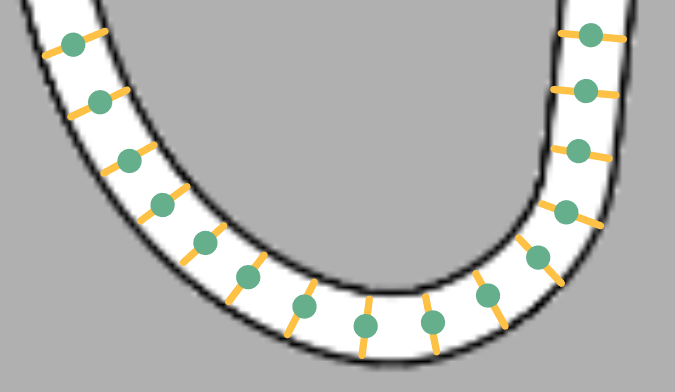
\includegraphics[width=0.65\textwidth]{centerline-ex.png}
	\end{center}
	\caption{La figura mostra la rappresentazione discreta della centerline (i punti verdi) e le linee
		immaginarie (quelle gialle) che uniscono, ortogonalmente rispetto alla centerline, i bordi
		del circuito}
		\label{fig:centerline-ex}
\end{figure}

\paragraph{Definizione di raceline}
\label{par:raceline}
I samples della raceline vengono calcolati a partire da quelli delle centerline "muovendoli" sulla linea
immaginaria che unisce i due bordi. Formalmente:
\[
	\overrightarrow{r_i} = \overrightarrow{p_i} + \alpha_i \overrightarrow{n_i}
\]
dove il sample $i$ della raceline $r$, descritto dal vettore $\overrightarrow{r_i}$, viene traslato di un
fattore $a_i$ lungo il vettore $\overrightarrow{n_i}$, ovvero la linea che unisce i bordi del circuito.
La figura \ref{fig:raceline-def} rappresenta graficamente questo processo.

\begin{figure}[h]
	\begin{center}
		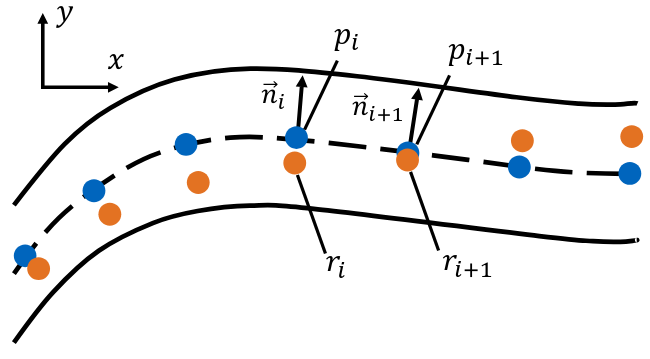
\includegraphics[width=0.75\textwidth]{raceline-def.png}
	\end{center}
	\caption{Rappresentazione grafica della raceline, dove i punti blu rappresentano i samples della
		centerline, mentre quelli arancioni sono quelli della raceline, traslati di un certo fattore lungo i
		vettori $n$ corrispondenti. \cite{lection22}}
	\label{fig:raceline-def}
\end{figure}

È necessario, inoltre, imporre un vincolo sul fattore $a$ in modo tale che non venga prodotto un sample
al di fuori del circuito o che non permetta al robot di passare perché troppo vicino ai bordi.
Formalmente:
\begin{equation}
	a_i \in [ -w_{tr\_left, i} + \frac{w_{veh}}{2}, w_{tr\_right, i} - \frac{w_{veh}}{2}]
	\label{eq:a_constr}
\end{equation}
dunque, dato un indice $i$, il fattore $a$ deve rientrare nel range definito tra la distanza del circuito
a sinistra $w_{tr\_left}$ del sample della centerline dello stesso indice e la distanza a destra
$w_{tr\_right}$ aggiustato per la larghezza del veicolo $w_{veh}$.

% ================== Path Planning =====================================
\section{Path planning}
\label{sec:path-models}
Ora verranno esaminate più in dettaglio il modello dei problemi di QP
geometrico per le strategie di percorso più breve e minor curvatura.

La programmazione quadratica è un processo che risolve problemi di ottimizzazione matematica descritti da
funzioni quadratiche. L'obiettivo è quello di trovare un vettore che minimizzi o massimizzi il valore di
una funzione obiettivo preservando contemporaneamente dei vincoli, descritti da disequazioni.

\paragraph{Percorso più breve}\cite{race-model}\cite{globalplanning-lec}
Il modello in questione deve descrivere il percorso più breve, ovvero che abbia la distanza minore tra i
samples. Un sample della raceline viene formulato come:
\[
	\overrightarrow{P_i} =
	\begin{bmatrix}
		x_{r,i} + a_i(x_{l,i} - x_{r,i}) \\
		y_{r,i} + a_i(y_{l,i} - y_{r,i})
	\end{bmatrix} =
	\begin{bmatrix}
		x_{r,i} + a_i\Delta_{x,i} \\
		y_{r,i} + a_i\Delta_{y,i}
	\end{bmatrix}
\]
ovvero, il punto più a destra del segmento $i$-esimo ortogonale alla centerline spostato sullo stesso per
un fattore $a$. Nella figura \ref{fig:short-path-expl} ne viene mostrato un esempio.\\
La distanza tra un sample e il suo successivo può essere descritta, quindi, come:
\[
	\Delta P_{x, i} = \overrightarrow{P}_{i+1} - \overrightarrow{P_i} = \begin{bmatrix}
		x_{r,i+1} - x_{r,i} + a_{i+1}\Delta_{x,i+1} - a_i\Delta_{x, i} \\
		y_{r,i+1} - y_{r,i} + a_{i+1}\Delta_{y,i+1} - a_i\Delta_{y, i}
	\end{bmatrix}
\]
Le variabili da trovare è il vettore di $a$ da applicare ai samples, dunque:
\[
	\begin{aligned}
		min\ [a_i \dots a_N] & \sum_{i=1}^{N} (\Delta P_{x,i})^2                          \\
		\text{subj. to}\     & a_i \in [a_{i, min}, a_{i, max}] \quad \forall 1 <= i <= N
	\end{aligned}
\]
dove il vincolo per $a_i$ è lo stesso descritto nella formula \ref{eq:a_constr}.

\begin{figure}[h]
	\begin{center}
		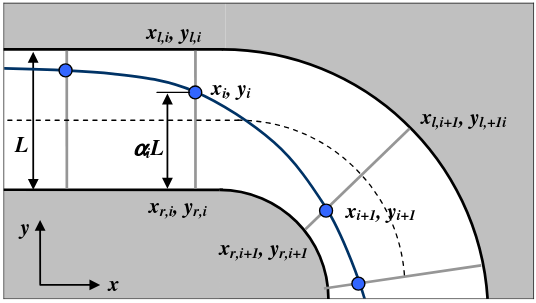
\includegraphics[width=0.65\textwidth]{short-path-expl.png}
	\end{center}
	\caption{Rappresentazione grafica della descrizione matematica di un sample. \cite{race-model}}
	\label{fig:short-path-expl}
\end{figure}

\paragraph{Minima Curvatura}
La formulazione del modello è identica a differenza, ovviamente, della funzione obiettivo che deve
descrivere la curvatura della raceline, il modello, quindi, viene definito come:
\[
	\begin{aligned}
		min\ [a_i \dots a_N] & \sum_{i=1}^{N} \kappa_i^2                                  \\
		\text{subj. to}\     & a_i \in [a_{i, min}, a_{i, max}] \quad \forall 1 <= i <= N
	\end{aligned}
\]
dove $\kappa_i$ è la curvatura della funzione in un sample $i$, definita come:
\[
	\kappa_i = \frac{{x'_i} {y''_i} - y'_i x''_i}{({x'_i}^2 + {y'_i}^2)^\frac{3}{2}}
\]
che elevata al quadrato:
\[
	\kappa_i^2 = \frac{{x'_i}^2 {y''_i}^2 - 2 x'_i x''_i y'_i y''_i + {y'_i}^2 {x''_i}^2}{({x'_i}^2 + {y'_i}^2)^3}
\]

% ================== Velocity Planning =================================
\section{Velocity planning}
\label{sec:velocity-plan}
Come citato precedentemente, il calcolo della velocità per ogni sample può essere calcolato con
l'algoritmo \textit{forward-backward}, che ha il vantaggio di essere semplice, veloce e sufficientemente
accurato.

L'algoritmo assume che il robot venga guidato ai suoi limiti fisici per ogni punto del percorso, quindi
si ha che l'accelerazione longitudinale dipende dai limiti del motore e dall'azione frenante dei freni,
mentre l'accelerazione laterale è limitata dalle forze massime trasmissibili degli pneumatici.

Ad alto livello, l'algoritmo si può riassumere in:
\begin{enumerate}
	\item Si genera una prima stima della velocità basandosi sulla massima accelerazione laterale per la
	      curvatura di ogni sample;
	\item Si riducono le stime alla velocità massima consentita per quei sample che la superano;
	\item \textbf{Forward}: si itera sui samples e, se non si sono superati i limiti fisici del robot, si
		applica una possibile accelerazione longitudinale, altrimenti
	\item \textbf{Backward}: si itera sui samples e si applica una possibile decelerazione longitudinale.
\end{enumerate}
In particolare per gli ultimi due punti la velocità al punto successivo viene calcolata come segue:
\begin{enumerate}

	\item \raggedright Si calcola l'accelerazione laterale data la curvatura per quel sample:\\
	      \centering $a_{y,i} = v_i^2 \cdot \kappa_i$ 

	\raggedright
	\item Si determina il potenziale rimanente per l'accelerazione longitudinale:\\
	      \begin{center}
			  $a_{x,i} = a_{x,max} \sqrt{\displaystyle 1- \left(\frac{a_{y,i}}{a_{y,max}}\right)^2}$
		  \end{center}

	\item Si può calcolare quindi la velocità al punto successivo assumendo un'accelerazione costante per
		la distanza $l_i$ tra un sample e quello successivo:\\
		\centering $v_{i+1} = \sqrt{v_i^2 + 2 \cdot a_{x,i} \cdot l_i}$
\end{enumerate}

% Chapter 4
% ======================================================================
% col: 20

\chapter{Implementazione}
\label{chap:impl}
In questo capitolo verranno descritti i passaggi implementati per generare la raceline ottima data una
mappa.

Nel corso dello studio di questa tesi, è stato integrato un fork
\footnote{https://github.com/CL2-UWaterloo/Raceline-Optimization} della repository ufficiale del paper
citato \cite{christ2021time}, utilizzandolo come base di partenza. Si è condotta un'analisi del codice
sorgente, identificando le parti rilevanti per lo scopo e apportando delle modifiche e
personalizzazioni per adattarlo al contesto. Questo ha permesso di ottimizzare le funzionalità
esistenti e di implementare ulteriori miglioramenti, garantendo così che il codice rispondesse alle
necessità dello studio.

\bigskip
\noindent I passaggi ad alto livello sono i seguenti:
\begin{enumerate}
	\item ottenere l'immagine di una mappa (per esempio attraverso \hyperref[par:slam]{SLAM});
	\item eventualmente ripulirla di imperfezioni e ottenere un circuito chiuso; 
	\item generare la centerline e calcolare la larghezza del circuito;
	\item applicare gli algoritmi di generazione della raceline;
\end{enumerate}
%TODO:spiegare occupancy grid?
La mappa viene digitalizzata in file immagine che rappresenta una \textit{occupancy grid}, mentre i
percorsi, che siano raceline o centerline, sono in formato csv con due colonne rappresentanti la
posizione $(x,y)$ di ogni sample, nel caso sia una centerline, e una terza colonna per la velocità per
quanto riguarda la raceline ed eventualmente ulteriori colonne per altri valori come l'accelerazione e
l'angolo di sterzata.
\newpage
Di seguito si indicano le specifiche della macchina usata durante questa tesi:
\begin{itemize}
	\item[-] \textit{OS}: Ubuntu 22.04.4 LTS (Jammy Jellyfish)
	\item[-] \textit{Kernel}: 6.8.0-40 generic x86\_64
	\item[-] \textit{CPU}: Intel Core i7-6700k quad core
	\item[-] \textit{RAM}: 16GB
\end{itemize}

\section{Generazione centerline}
Affinché l'algoritmo per l'estrazione della linea di riferimento restituisca un risultato corretto, come
detto in precedenza, l'immagine della mappa deve rappresentare un circuito chiuso e con bordi ben
definiti e lisci, come effettivamente sarebbe un circuito di F1.
Dunque se si acquisisce una mappa con SLAM come in figura \ref{fig:slam_map} è necessario modificarla come
in figura \ref{fig:slam_map_mod}. Durante l'implementazione di questa tesi si è deciso di usare le mappe
dei circuiti da gara più famosi forniti da F1TENTH stesso \cite{f1tenth-gitmaps}.

\begin{figure}[H]
	\begin{minipage}[c]{0.47\textwidth}
		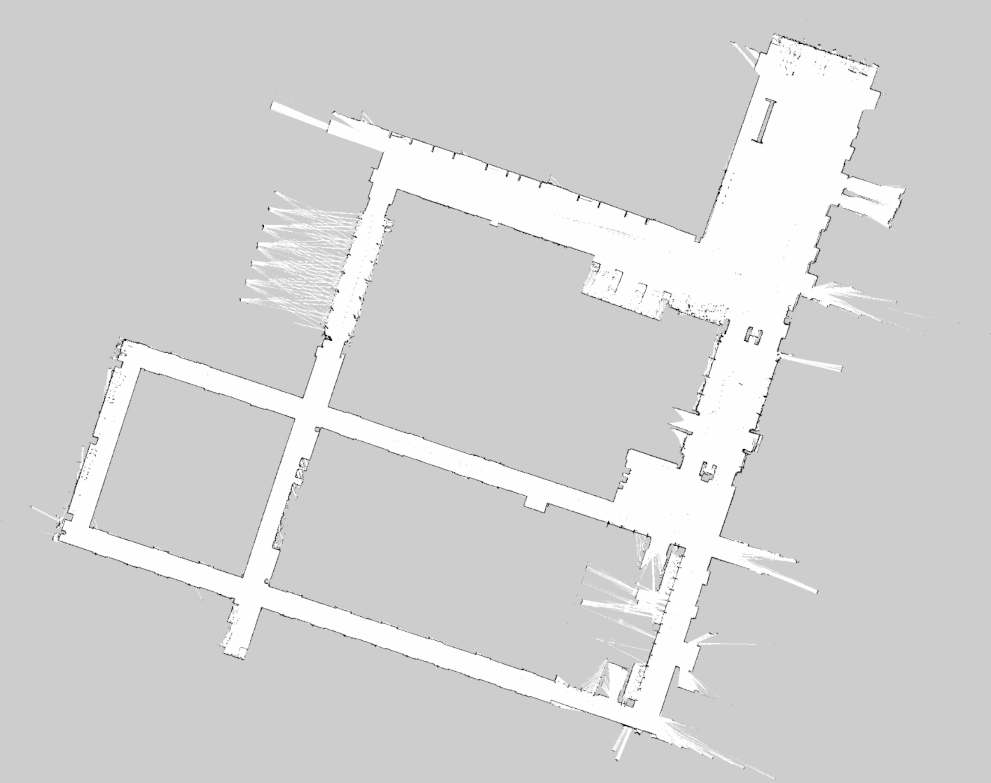
\includegraphics[width=1\textwidth]{slam_map.png}
		\caption{\raggedright Mappa risultante da SLAM \cite{stevengong} }
		\label{fig:slam_map}
	\end{minipage}\hfill
	\begin{minipage}[c]{0.47\textwidth}
		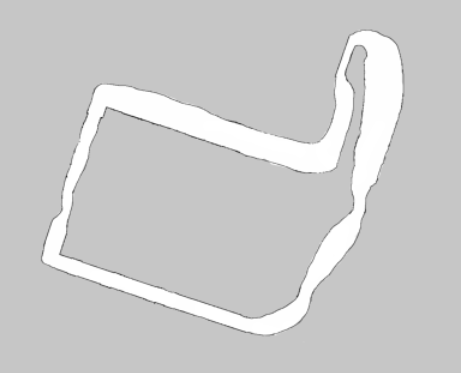
\includegraphics[width=1\textwidth]{slam_map_mod.png}
		\caption{Modifica dell'immagine \ref{fig:slam_map} per creare un circuito chiuso \cite{stevengong} }
		\label{fig:slam_map_mod}
	\end{minipage}
\end{figure}

Operativamente, l'algoritmo usato per la generazione viene dal mondo dell'elaborazione delle immagini e
si chiama EDT (Euclidian Distance Transform), che calcola la distanza euclidea per ogni pixel
dell'immagine dal background: in questo caso, lo sfondo preso in considerazione sono i punti non
esplorati, ovvero quelli esterni ai bordi del circuito.
Un esempio di applicazione di EDT si trova all'immagine \ref{fig:edt-ex}.

Un aspetto da sottolineare è che le immagini fornite da F1TENTH rappresentano una occupancy grid
ternaria, in cui il grigio corrisponde alle zone non esplorate; per sfruttare l'algoritmo sopra citato è
necessario che i pixel grigi vengano convertiti in nero, perché  è il valore considerato come background
dall'algoritmo EDT. Prendendo come riferimento il circuito di Monza all'immagine \ref{fig:monza-binary}, il
risultato dell'algoritmo si può vedere all'immagine \ref{fig:monza-edt}.

\begin{figure}[H]
	\begin{center}
		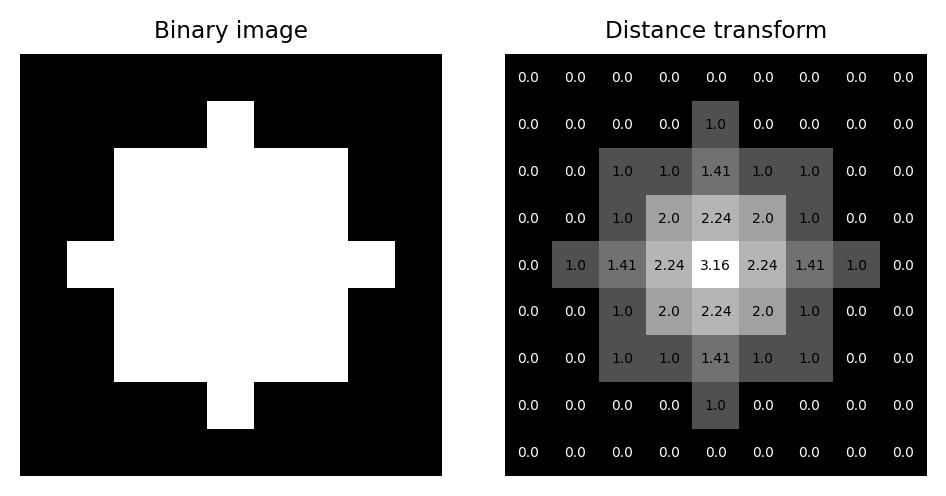
\includegraphics[width=1\textwidth]{edt-ex.png}
		\caption{Esempio di applicazione dell'algoritmo EDT su una immagine binaria, l'immagine a destra
		mostra il risultato indicando la distanza euclidea dal background per ogni pixel \cite{stevengong-edt} }
		\label{fig:edt-ex}
	\end{center}
\end{figure}
\begin{figure}[H]
	\begin{minipage}[c]{0.47\textwidth}
		
\includegraphics[width=1\textwidth]{monza-binary.png}
		\caption{Immagine della occupancy grid binaria del circuito di Monza}
		\label{fig:monza-binary}
	\end{minipage}\hfill
	\begin{minipage}[c]{0.47\textwidth}
		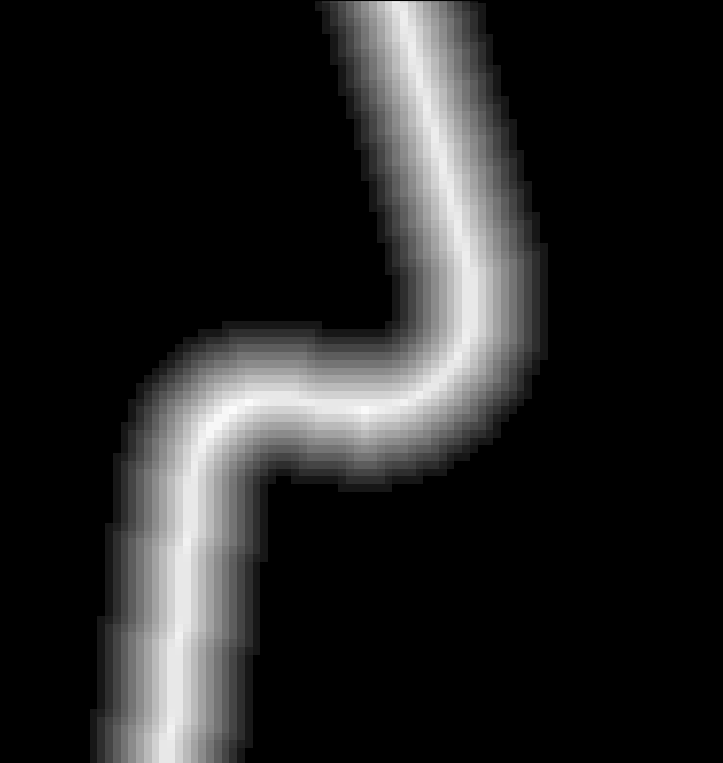
\includegraphics[width=1\textwidth]{monza-edt.png}
		\caption{\raggedright Risultato dell'algoritmo EDT mostrato sulla curva 1-2 del circuito di Monza}
		\label{fig:monza-edt}
	\end{minipage}
\end{figure}

Il passo successivo è quello di ottenere solo la parte centrale, ovvero quella con i valori di bianco
più alti e ridurla a un singolo pixel. In Python, questa operazione, viene eseguita dalla funzione
\verb|skeletonize()| del pacchetto \verb|scikit-image|. Seguendo l'esempio con il circuito di Monza, il
risultato di questa fase si può osservare all'immagine \ref{fig:monza-skel}.

A questo punto è necessario campionare il percorso di un pixel trovato: partendo da un punto del
percorso, si applica una ricerca DFS (Depth First Search) per trovare i successivi pixel bianchi. Dunque
da un pixel del percorso, si cerca il primo pixel bianco in tutte le direzioni che non sia già stato
esplorato: seguendo questo processo si ottengono le posizioni dei pixel e la loro distanza dai bordi, si
trasformano nel frame della mappa e esportano queste informazioni in un csv contenente le colonne
\verb|x, y, width_left, width_right|.
\vfill
\begin{figure}[h]
	\begin{center}
		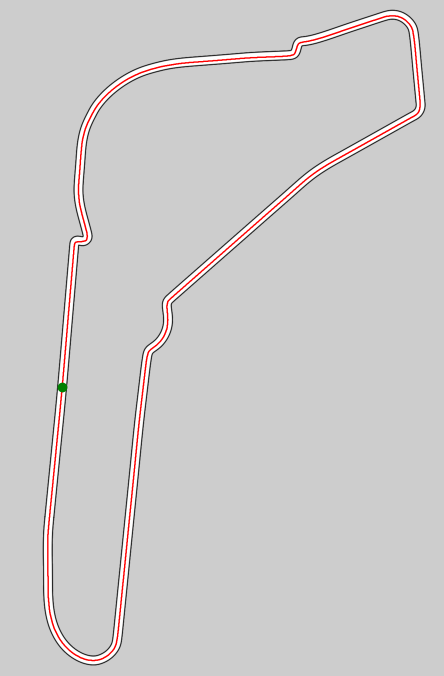
\includegraphics[width=0.6\textwidth, angle=90]{monza-skel.png}
	\end{center}
	\caption{Visualizzazione della centerline di Monza, il punto verde indica il punto di partenza}\label{fig:monza-skel}
\end{figure}

\newpage

%TODO: parlare di cosa produce (il csv)

\section{Esecuzione dell'ottimizzazione}
Ad alto livello, l'ottimizzazione cerca iterativamente di aggiustare la centerline in modo tale da
ottenere il risultato migliore, come spiegato nel capitolo \ref{chap:opt} (pag. \pageref{chap:opt}).
Questa fase non richiede solamente di eseguire il programma solutore, ma è necessario
configurare i parametri che l'algoritmo usa. Questo compito si chiama \textit{tuning} dei parametri
e consiste nel trovare quelli che meglio si adattano nel trovare la soluzione migliore.

Durante lo studio di questa tesi il principale parametro modificato durante le prove è stato lo
\textit{stepsize}, ovvero la distanza, in metri, tra un sample e l'altro. In particolare si distinguono
tre stepsize diversi:
\begin{itemize}
	\item \verb|stepsize_prep|: viene usato per l'interpolazione lineare prima dell'approssimazione del
		percorso con la spline;
	\item \verb|stepsize_reg|: usato durante l'ottimizzazione per l'interpolazione della spline;
	\item \verb|stepsize_interp_after_opt|: usato per campionare la spline dopo l'ottimizzazione, è la
		distanza dei sample esportati nel csv risultante;
\end{itemize}
Altri parametri fanno riferimento alla dinamica del veicolo, come angolo di sterzata massimo e velocità
massima, e grandezze fisiche del veicolo, come massa, lunghezza e larghezza. Sono disponibili anche
parametri specifici per il tipo di ottimizzazione, per esempio un valore aggiuntivo alla larghezza del
veicolo che comprende un margine di sicurezza dai bordi del circuito. Di seguito si mostrano alcuni dei
valori usati che descrivono le proprietà del veicolo indipendentemente dal tipo di ottimizzazione usato:

\begin{lstlisting}
veh_params = {
	"v_max": 15.0,       # [m/s]
	"length": 0.58,      # [m]
	"width": 0.31,       # [m]
	"mass": 3.74,        # [Kg]
	"dragcoeff": 0.075,  # [kg*m^2/m^3]
	"curvlim": 3.0,      # [rad/m]
	"g": 9.81            # [N/Kg]
}
\end{lstlisting}

\begin{figure}[h]
	\begin{center}
		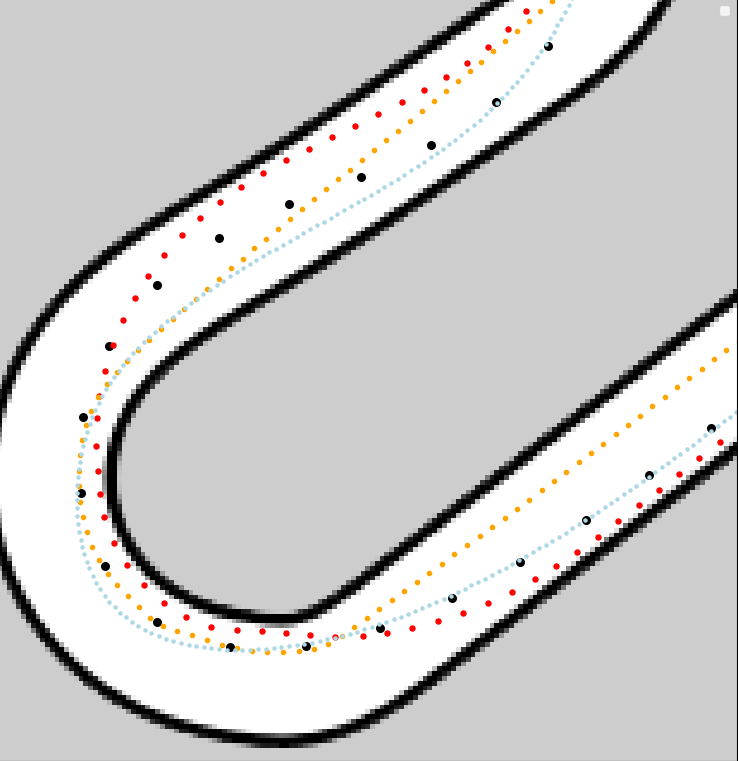
\includegraphics[width=0.75\textwidth]{stepsize.png}
	\end{center}
	\caption{Quattro traiettorie con stepsize diversi: nera a 1.5m, rossa a 0.5m,
	arancione a 0.3m e azzurra a 0.15m}
	\label{fig:stepsize}
\end{figure}

\subsection{Tuning dei parametri}
\label{par:tuning}
È facile immaginare che una minore distanza tra i sample durante l'ottimizzazione porti un risultato
più preciso a costo di aumentare il tempo di esecuzione. %, come dimostrato nel capitolo successivo. % TODO: fare riferimento all'analisi
In figura \ref{fig:stepsize} si visualizza una comparazione tra raceline con stepsize diversi.

Come ci si potrebbe aspettare, il parametro che controlla principalmente il tempo di esecuzione è lo
stepsize durante l'ottimizzazione, ovvero \verb|stepsize_reg|, per questo è stato necessario scegliere un
valore tale che bilanci bene la qualità del tracciato prodotto e il tempo di esecuzione. Infatti, per
evitare che l'ottimizzazione impieghi troppo tempo, il numero di iterazioni è limitato a 2000: se entro
questo limite non è stata trovata una soluzione viene ritornato un errore.

In linea generale, si è riscontrato che:
\begin{itemize}
	\item \verb|stepsize_prep|, per quanto riguarda il percorso più breve e la curvatura minima, impatta
		sulla qualità del risultato, diversamente dal tempo minimo; non influisce significativamente sul
		tempo di esecuzione. Valori in $[0.1, 0.5)$ per i primi due, $[0.5, 1]$ per mintime;
	\item \verb|stepsize_reg|, come accennato precedentemente, incide sul tempo di esecuzione
		e in modo apprezzabile per mintime; è significativo per la qualità del percorso. Valori $ > 0.3$
		per shortest path e mincurv, mentre per mintime sono necessari valori $> 1.0$ per evitare di
		sforare le 2000 iterazioni;
	\item \verb|stepsize_interp_after_opt| non incide in modo sostanziale sul tempo e per questo può
		essere valorizzato in base alle necessità dell'algoritmo che userà il percorso.
\end{itemize}
A valori alti degli stepsize (es: $> 1.5$), può capitare che la raceline generata "tagli" il percorso per
curve molto rapide, come nella chicane di Spa. Questo è capitato principalmente con l'algoritmo del
percorso più breve, come mostrato alla figura \ref{fig:taglio-spa}

\begin{figure}[h]
	\begin{minipage}[c]{0.45\textwidth}
		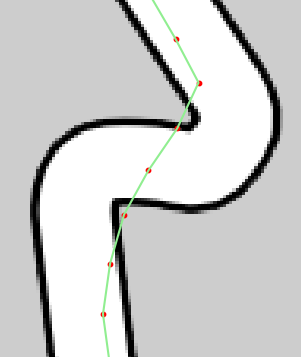
\includegraphics[width=0.3\textheight]{chicane_shpth.png}
		\caption{Generazione errata del percorso per via di stepsize troppo ampi}
		\label{fig:taglio-spa}
	\end{minipage}\hfill
	\begin{minipage}[c]{0.45\textwidth}
		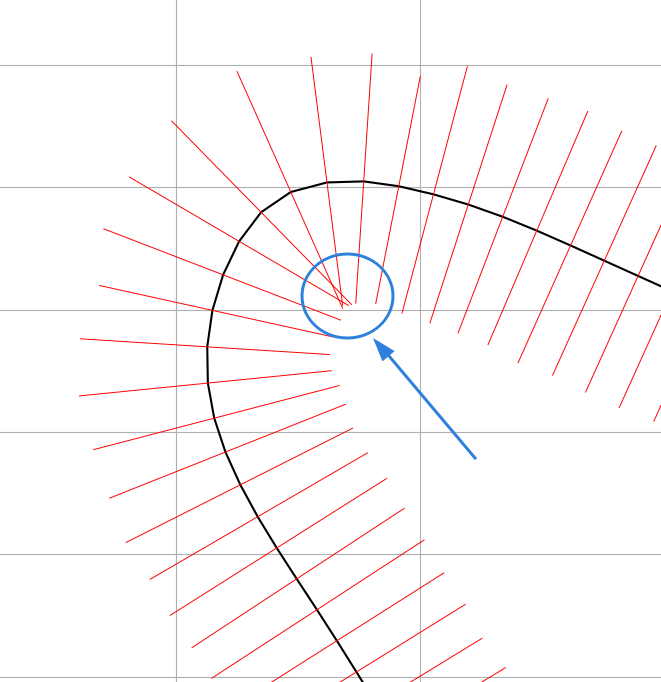
\includegraphics[width=\textwidth]{nomral-crossed.png}
		\caption{\raggedright Linee ortogonali alla centerline incrociate}
		\label{fig:norm-cross}
	\end{minipage}
\end{figure}
Altri parametri modificati durante le sperimentazioni sono qualità inerenti alle spline, principalmente
lo smoothing factor. Quest'ultimo, se troppo basso e in concomitanza con valori di stepsize bassi, può
generare delle linee ortogonali che si incrociano tra loro e che quindi non possono produrre un percorso
corretto. Un esempio di questo caso è visibile all'immagine \ref{fig:norm-cross}. Durante le
sperimentazioni questo valore è stato fissato a 80.
\newpage
\noindent Di seguito si mostrano gli stepsize usati per generare il percorso a figura \ref{fig:taglio-spa}.
\begin{lstlisting}
stepsize_opts={
	"stepsize_prep": 1.0,
	"stepsize_reg": 1.5,
	"stepsize_interp_after_opt": 1.5
}
\end{lstlisting}
Mentre i successivi sono i parametri della spline e stepsize utilizzati per la figura \ref{fig:norm-cross}.

\begin{lstlisting}
stepsize_opts={
	"stepsize_prep": 0.1,
	"stepsize_reg": 0.5,
	"stepsize_interp_after_opt": 0.3
}

reg_smooth_opts={
	"k_reg": 3,   # grado della spline
	"s_reg": 1.0  # smoothing factor [1.0, 100]
}
\end{lstlisting}

% Chapter 5

\chapter{Analisi dei risultati}


\printbibliography
\end{document}
